\chapter{函数空间}
\label{chap:function-spaces}
\label{chap:functional-analysis-and-approximation}

拟合一条曲线时，我们常把候选写成固定基函数的组合$f_m=\sum_{j=1}^mc_j\varphi_j$，并用系数向量的欧氏距离比较两个候选。只要$m$固定、基也固定，这样做没有问题。可是一旦为了提高精度而不断增加项数，系数向量的维数随之改变；同一个函数换一组基，系数也会完全不同。这时“两条函数相差多少”“一列近似是否收敛”“极限还是不是我们要的那类函数”，都不能再靠比较系数回答，而要直接在函数之间建立距离和几何。

本章围绕四个问题展开：哪些函数可以参与线性运算，什么情况下两个函数算作同一个元素？怎样规定两条函数之间的误差？一列彼此越来越接近的函数，极限是否仍在原来的函数集合里？在有了内积之后，能否像在有限维中那样取出最近分量，并用正交方向写出坐标？

第~\ref{sec:fs-elements}节先确定空间的成员和“相等”的含义：逐点运算使函数组成线性空间，积分误差则要求把只在零测集上不同的函数看成同一个元素。第~\ref{sec:fs-norms-completeness}节在这些元素上建立范数、完备性和内积，并用连续斜坡逼近阶跃的例子说明，各项互相接近并不保证极限留在原集合中。这个例子贯穿后文：第~\ref{sec:fs-continuous}节表明同一组连续函数在一致范数下完备，换成平方积分误差就不完备；第~\ref{sec:fs-integral}节因此扩大到可测函数的等价类，构造$L^p$空间并证明它们完备。

有了多种空间，第~\ref{sec:fs-relations}节比较它们：成员何时能从一个空间转入另一个，换一个测度后元素与误差怎样变化，哪些简单函数足以逼近一般成员，以及一致、积分和逐点三种收敛之间能推出什么、不能推出什么。第~\ref{sec:fs-orthogonal}节回到Hilbert空间，证明闭子空间上的正交投影存在且唯一，并用正交系写出展开和截断误差；斜坡与阶跃的例子在这里再次出现，说明闭性缺失时最近点可能不存在。

全章以实值函数为主线，复数情形只在需要时补充约定。所用的测度、积分及其极限定理来自第~\ref{chap:measure-spaces}章，完备性、稠密性和可分性的一般定义来自第~\ref{chap:metric-spaces}章；本章把它们落实到函数上，不重新组织积分论。

% 第1章第1节：函数作为空间元素（线性运算与维数；普通函数与几乎处处等价类）。

\section{函数作为空间元素}
\label{sec:fs-elements}

要比较两条函数、讨论一列函数的极限，先得说清楚参与比较的对象是什么。本节回答两个问题：函数之间怎样做加法和数乘，一个函数集合何时对这些运算封闭；以及在积分误差下，什么样的两个函数应当看成同一个元素。后面所有的范数、点值和极限都沿用这里的约定。

\subsection{函数的线性运算与维数}
\label{sec:fs-linear-structure}

\paragraph{逐点运算}
固定一个非空的输入集合$X$，考虑实值函数$f:X\to\mathbb R$。讨论函数时要分清三个层次：输入位置$x$，函数在该位置的值$f(x)$，以及整个函数$f$。前两者是$X$中的点和实数，第三者是一条完整的对应规则。本章把第三者当作一个“点”来处理。

两个函数的和与一个函数的数乘逐点定义：
\[
 (f+g)(x)=f(x)+g(x),\qquad (cf)(x)=c\,f(x),\qquad x\in X,\ c\in\mathbb R .
\]
每个等式右边都是实数运算，所以交换律、结合律、分配律等线性空间公理在每个$x$处分别成立，从而对整个函数成立；零元素是处处为零的函数，$f$的负元是$x\mapsto-f(x)$。于是全体函数$X\to\mathbb R$组成一个实线性空间。线性空间与线性子空间的一般定义可参考\BookChapterRef{chap:linear-representation}{卷一“线性空间、映射与坐标”章}。

\paragraph{子空间的封闭性检查}
实际使用的通常不是全体函数，而是某个候选集合$V$。要把$V$当作线性子空间，必须逐项核对：零函数在$V$中，$V$中两个成员之和仍在$V$中，成员的数乘仍在$V$中。闭区间$[a,b]$上的连续函数全体$C([a,b])$满足这三条，因为连续函数的和与数乘仍连续；次数不超过$m$的多项式全体$\mathcal P_m$也满足，因为两个这样的多项式相加不会提高次数。更一般地，任意给定函数$\varphi_1,\ldots,\varphi_m$的张成$\operatorname{span}\{\varphi_1,\ldots,\varphi_m\}$总是线性子空间。

由参数描述的函数族却不一定封闭。考虑单个“折线单元”组成的族
\[
 \mathcal R=\{\,x\mapsto a\max(0,x-t):a,t\in\mathbb R\,\},
\]
它只有两个参数。取$f(x)=\max(0,x)$与$g(x)=\max(0,x-1)$，二者都在$\mathcal R$中，但$f+g$在$x=0$和$x=1$各有一个折点，而$\mathcal R$中每个成员至多一个折点，所以$f+g\notin\mathcal R$。宽度固定的神经网络、固定节点数的样条等非线性参数族都有同样的现象：两个成员之和通常需要更多的参数才能表示。这类族可以作为逼近工具（第~\ref{chap:function-approximation}章），但不能直接当作线性空间使用。

\paragraph{输入维数、参数数目与空间维数}
函数空间的维数与输入的维数是两回事。在区间$[a,b]$上，函数$1,x,x^2,\ldots,x^m$线性无关：若$\sum_{k=0}^mc_kx^k=0$对每个$x\in[a,b]$成立，左边是一个在无穷多点取零的多项式，只能所有系数为零。$m$可以任意大，所以$C([a,b])$包含任意多个线性无关的方向，是无限维的，尽管输入只有一个坐标。

参数数目又是第三回事。上面的$\mathcal R$只有两个参数，却不是线性空间，谈不上维数；$\mathcal P_m$是$m+1$维空间，参数数目恰为维数。即使在同一个有限维空间里，坐标也依赖所选的基。例如$x^2$在基$\{1,x,x^2\}$下的系数是$(0,0,1)$，在基$\{1,x,x^2-\tfrac13\}$下的系数是$(\tfrac13,0,1)$。若用系数的欧氏距离衡量误差，同一对函数在两组基下会得到不同的数值；若为提高精度不断增加项数，系数向量更是落在维数不断变化的空间里。因此比较函数需要一个不依赖表示坐标、直接作用于函数本身的误差规则，这就是第~\ref{sec:fs-norms-completeness}节的范数。

\subsection{普通函数与几乎处处等价类}
\label{sec:fs-ae-classes}

\paragraph{零测改值}
逐点运算把每个函数都当作不同的元素：只要某一点的值改变，函数就变了。但若两个函数之间的误差是通过积分累计的，有些改动根本不影响误差。在$[0,1]$上取Lebesgue测度，令$f\equiv0$，而$g$除$g(\tfrac12)=1$外处处为零。单点集的Lebesgue测度为零，零测集上的改动不影响积分（第~\ref{sec:measure-general-structure}节），所以
\[
 \int_0^1|f(x)-g(x)|\,dx=0 .
\]
图~\ref{fig:fs-ae-representatives}显示了这两个函数：作为普通函数它们在$x=\tfrac12$处不同，但任何用积分衡量的误差都看不出差别。

\begin{figure}[!htb]
  \centering
  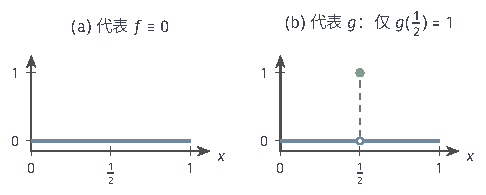
\includegraphics[width=82.2mm]{figures/02-abstract-mathematics/03-function-spaces/tikz/c1-ae-representatives/figure.pdf}
  \caption{同一个几乎处处等价类的两个代表。定义域为$[0,1]$并取Lebesgue测度；(a)中$f\equiv0$，(b)中$g$只在$x=\tfrac12$处取$1$（绿点），空心圈表示$g$在该点不取$0$。单点集测度为零，所以$\int_0^1|f-g|\,dx=0$，二者代表同一个积分空间元素，但它们在$\tfrac12$处的点值不同。}
  \label{fig:fs-ae-representatives}
\end{figure}

\paragraph{等价类与线性运算}
在测度空间$(X,\mathcal A,\mu)$上，对两个可测函数规定
\[
 f\sim_\mu g\quad\Longleftrightarrow\quad \mu(\{x:f(x)\neq g(x)\})=0,
\]
即$f=g$在$\mu$下几乎处处成立。这是一个等价关系：自反与对称是显然的；若$f\sim_\mu g$且$g\sim_\mu h$，则$\{f\neq h\}\subseteq\{f\neq g\}\cup\{g\neq h\}$，两个零测集的并仍是零测集，所以$f\sim_\mu h$。把与$f$几乎处处相等的可测函数全体记为$[f]_\mu$，称为$f$的\term{等价类}（equivalence class），$f$称为它的一个代表。

等价类之间的线性运算借助代表定义：$[f]_\mu+[g]_\mu=[f+g]_\mu$，$c[f]_\mu=[cf]_\mu$。要使这个定义有意义，结果必须不依赖代表的选择。若$f'\sim_\mu f$、$g'\sim_\mu g$，则
\[
 \{f'+g'\neq f+g\}\subseteq\{f'\neq f\}\cup\{g'\neq g\},
\]
右边是零测集，所以$f'+g'\sim_\mu f+g$；数乘同理。于是可测函数的等价类组成一个线性空间，零元素是“几乎处处为零的函数”这一整类。第~\ref{sec:fs-integral}节的$L^p$空间就建立在这样的等价类上。

\paragraph{点值不再自动有意义}
取等价类的代价是：一个类通常没有确定的点值。在Lebesgue测度下每个单点都是零测集，同一类中的代表可以在任意给定的点取任意值，所以“$[f]_\mu$在$x_0$处的值”没有意义。这与测度有关。若某点是原子，即$\mu(\{x_0\})>0$，则同一类的所有代表在$x_0$处必须取同一个值；在计数测度下只有空集是零测集，等价类退化为普通函数。

也不能把等价类当作已经选好了“最好的”代表。在区间上的Lebesgue测度下，若一个类含有连续代表，这个连续代表是唯一的：两个连续函数之差不为零的点组成开集，非空开区间的测度为正，所以两个几乎处处相等的连续函数必定处处相等。但许多类根本没有连续代表（第~\ref{sec:fs-norms-completeness}节的阶跃函数就是一例），而且即使有，从类中读出它的点值也需要另外的论证。本章只固定元素的含义；点值读取何时有良定义、何时连续，由第~\ref{sec:lfo-point-evaluation}小节讨论，点值读取连续的Hilbert函数空间则是第~\ref{chap:rkhs}章的对象。

% 第1章第2节：范数、内积与完备性（函数范数与误差；范数收敛与Banach空间；内积与Hilbert空间）。

\section{范数、内积与完备性}
\label{sec:fs-norms-completeness}

有限维向量的范数与内积在卷一中已经建立，本节把它们用到函数上。定义本身几乎不变，变化在于用途：在无限维空间里，一列彼此越来越接近的元素是否真有极限、极限是否还在原来的集合中，需要逐一检查，而不再像有限维那样自动成立。

\subsection{函数范数与误差}
\label{sec:fs-norms}

\paragraph{两种误差要求}
比较$[0,1]$上的$f(x)=x$与$g(x)=x^2$，至少有两种自然的做法。若关心最坏的位置，可以取最大偏差$\sup_{x}|x-x^2|$；$x-x^2$在$x=\tfrac12$处取最大值，结果为$\tfrac14$。若关心整体的累计偏差，可以取$\int_0^1|x-x^2|\,dx=\tfrac12-\tfrac13=\tfrac16$。两个数都合理，回答的是不同的问题。为了让不同的误差规则共享同一套推理，我们只要求它们满足几条共同的性质。

\begin{definition}[范数]
\label{def:fs-norm}
设$V$是实（或复）线性空间。映射$\|\cdot\|:V\to[0,\infty)$称为$V$上的\term{范数}（norm），若对所有$f,g\in V$与标量$c$，
\begin{enumerate}
 \item 正定性：$\|f\|=0$当且仅当$f=0$；
 \item 齐次性：$\|cf\|=|c|\,\|f\|$；
 \item 三角不等式：$\|f+g\|\leq\|f\|+\|g\|$。
\end{enumerate}
配备了范数的线性空间称为赋范空间。
\end{definition}

三条公理各有用处。正定性保证误差为零当且仅当两个元素相同；齐次性保证把函数整体放大$c$倍时误差也放大$|c|$倍；三角不等式保证两段误差串联起来不超过各自之和，这是后面所有误差估计的基本工具。令$d(f,g)=\|f-g\|$，由三条公理可以直接验证度量公理（定义~\ref{def:metric-space}）：例如$d(f,h)=\|(f-g)+(g-h)\|\leq d(f,g)+d(g,h)$。所以每个赋范空间都是度量空间，第~\ref{chap:metric-spaces}章关于收敛、Cauchy列、闭集和完备性的结论都可以直接使用。

\paragraph{半范数与零方向}
有时一个误差公式满足齐次性和三角不等式，却让某些非零元素的“长度”为零，这样的公式称为\term{半范数}（seminorm）。在$[0,1]$上的全体有界可积函数中，$p(f)=\int_0^1|f|\,dx$就是半范数：上一节的$g=\mathbf 1_{\{1/2\}}$不为零，却有$p(g)=0$。又如在连续可微函数上，$p(f)=\sup_x|f'(x)|$对所有常数函数都取零。

处理零方向有两种办法。一是缩小对象：把$\int_0^1|f|\,dx$限制在$C([0,1])$上，若连续函数$f$在某点$x_0$处$|f(x_0)|>0$，则在$x_0$的一个邻域内$|f|>|f(x_0)|/2$，积分为正，所以在连续函数上它是范数。二是把零长度的元素识别为零，即对半范数为零的方向取商；在积分误差下，这正是第~\ref{sec:fs-ae-classes}小节的几乎处处等价类。第~\ref{sec:metric-pseudometric}节在度量空间中讨论过同样的商构造。无论哪种办法，都不能直接把只满足半范数条件的公式称为原对象上的范数。

\paragraph{系数误差与Gram矩阵}
回到章首的问题：当函数由有限个基函数表示时，函数之间的误差和系数之间的误差是什么关系？取平方积分误差$\|h\|_2^2=\int h^2\,d\mu$。对$f=\sum_jc_j\varphi_j$与$g=\sum_jc'_j\varphi_j$，记$\bm\delta=\bm c-\bm c'$，展开平方并利用积分的线性，
\[
 \|f-g\|_2^2=\int\Bigl(\sum_{i}\delta_i\varphi_i\Bigr)\Bigl(\sum_j\delta_j\varphi_j\Bigr)d\mu
 =\sum_{i,j}\delta_i\delta_j\int\varphi_i\varphi_j\,d\mu
 =\bm\delta^{\top}\bm G\bm\delta,
\]
其中$\bm G_{i,j}=\int\varphi_i\varphi_j\,d\mu$组成\term{Gram矩阵}（Gram matrix）。系数的欧氏距离平方是$\bm\delta^{\top}\bm\delta$，两者相等当且仅当$\bm G=\bm I$，即基函数两两正交且各自的平方积分为$1$。

在$[-1,1]$上取Lebesgue测度与基$\{1,x\}$，$\int1\,dx=2$，$\int x\,dx=0$，$\int x^2\,dx=\tfrac23$，所以$\bm G=\operatorname{diag}(2,\tfrac23)$，函数误差为$2\delta_1^2+\tfrac23\delta_2^2$。系数差$(1,0)$与$(0,1)$的欧氏长度都是$1$，对应的函数误差却分别是$\sqrt2$与$\sqrt{2/3}$。若改在$[0,1]$上使用同一组基，$\bm G=\begin{bmatrix}1&1/2\\1/2&1/3\end{bmatrix}$不再是对角阵，常数方向与线性方向的误差还会相互耦合。平方积分误差在连续函数上确实是范数：正定性的论证与上一段相同，三角不等式由Cauchy--Schwarz不等式得到，下面第~\ref{sec:fs-hilbert}小节在一般内积空间中给出证明。有限维的Gram矩阵、正交化与范数等价，可参考\BookChapterRef{chap:normed-inner-product-spaces}{卷一“赋范空间与内积空间”章}；本章不重建这些结论。

\subsection{范数收敛与Banach空间}
\label{sec:fs-banach}

有了范数，就可以讨论函数列的收敛。设$(f_n)$是赋范空间$V$中的序列，$f\in V$。若$\|f_n-f\|\to0$，称$f_n$\term{依范数收敛}（convergence in norm）到$f$。若对每个$\varepsilon>0$存在$N$，使$m,n\geq N$时$\|f_n-f_m\|<\varepsilon$，称$(f_n)$为范数意义下的\term{Cauchy列}（Cauchy sequence）。由三角不等式$\|f_n-f_m\|\leq\|f_n-f\|+\|f-f_m\|$，收敛列一定是Cauchy列。反过来是否成立，取决于空间。

\paragraph{斜坡逼近阶跃}
在$C([-1,1])$上使用平方积分范数$\|g\|_2=\bigl(\int_{-1}^1g^2\,dx\bigr)^{1/2}$，考察连续斜坡
\[
 g_n(x)=\begin{cases}-1,&x\leq-1/n,\\ nx,&|x|<1/n,\\ 1,&x\geq1/n,\end{cases}\qquad n\geq1 .
\]
图~\ref{fig:fs-ramp-step}画出了$g_2,g_4,g_{16}$：斜坡越来越陡，越来越像阶跃函数$\operatorname{sgn}$。我们先验证它们组成Cauchy列。设$m>n$。在$|x|\geq1/n$处$g_n=g_m$；在$|x|<1/n$处二者同号且绝对值不超过$1$，所以$|g_n-g_m|\leq1$。于是
\[
 \|g_n-g_m\|_2^2\leq\int_{-1/n}^{1/n}1\,dx=\frac2n\to0 .
\]

\begin{figure}[!htb]
  \centering
  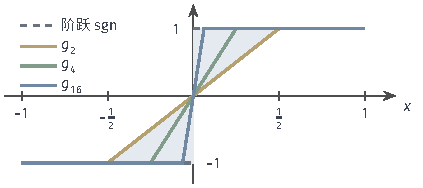
\includegraphics[width=71.6mm]{figures/02-abstract-mathematics/03-function-spaces/tikz/c1-ramp-step/figure.pdf}
  \caption{连续斜坡$g_n$逼近阶跃$\operatorname{sgn}$。$g_n$在$|x|\geq1/n$处与$\operatorname{sgn}$相同，只在宽为$2/n$的区间内线性过渡；阴影是$n=2$时二者的差所在的区域。直接积分得$\int_{-1}^1(g_n-\operatorname{sgn})^2\,dx=\tfrac{2}{3n}\to0$，但$\operatorname{sgn}$在$0$处跳跃，没有连续代表。}
  \label{fig:fs-ramp-step}
\end{figure}

接下来证明这列函数在$C([-1,1])$中没有$\|\cdot\|_2$极限。假设存在连续函数$g$使$\|g_n-g\|_2\to0$。任取$\delta\in(0,1)$，当$n>1/\delta$时$g_n$在$[\delta,1]$上恒为$1$，所以
\[
 \int_\delta^1(1-g)^2\,dx\leq\int_{-1}^1(g_n-g)^2\,dx\to0 .
\]
左边不依赖$n$，只能为零；$(1-g)^2$连续且非负，故$g=1$在$[\delta,1]$上处处成立。同理$g=-1$在$[-1,-\delta]$上成立。由于$\delta$任意，$g$在$(0,1]$上恒为$1$、在$[-1,0)$上恒为$-1$，在$0$处不可能连续，矛盾。

这个例子把两件事分开了：“各项互相接近”是序列自身的性质，“在给定的集合中存在极限”则同时取决于集合和范数。直观上，$g_n$的“极限”应该是阶跃函数，只是阶跃函数不在$C([-1,1])$中。

\begin{definition}[Banach空间]
\label{def:fs-banach}
若赋范空间$V$中的每个Cauchy列都依范数收敛到$V$中的某个元素，称$V$是\term{完备}（complete）的。完备的赋范空间称为\term{Banach空间}（Banach space）。
\end{definition}

按此定义，$(C([-1,1]),\|\cdot\|_2)$不是Banach空间。完备性同时依赖候选集合和范数：第~\ref{sec:fs-uniform-norm}小节将证明同一个$C([-1,1])$在最大偏差范数下完备，第~\ref{sec:fs-lp-completeness}小节则把集合扩大为可测函数的等价类，使平方积分范数下的极限有处可去。

\paragraph{闭子空间与完备性}
在已经完备的空间里，子空间是否完备由它是否闭决定。第~\ref{sec:metric-convergence-completeness}节对度量空间证明了：完备空间的闭子集是完备的，完备子集一定是闭的（定理~\ref{thm:metric-complete-closed}）。用在Banach空间$X$的线性子空间$M$上，这两句话的分工很清楚：$X$的完备性保证$M$中的Cauchy列在$X$中有极限，$M$的闭性保证这个极限没有跑出$M$。

多项式给出一个不闭的子空间。在$[0,1]$上用最大偏差衡量误差，$e^x$的Taylor多项式$p_N(x)=\sum_{k=0}^Nx^k/k!$满足
\[
 \sup_{x\in[0,1]}|e^x-p_N(x)|\leq\frac{e}{(N+1)!}\to0,
\]
这是Lagrange余项的估计。所以$p_N$是多项式空间中的Cauchy列，在连续函数空间中的极限是$e^x$，而$e^x$不是多项式（它的各阶导数都不恒为零）。多项式空间因此不闭，也不完备。第~\ref{sec:apx-polynomial}小节将说明，多项式在这个范数下可以逼近任意连续函数，即它的闭包是整个$C([0,1])$。

\paragraph{完备化}
不完备的空间可以通过添加极限补全。第~\ref{sec:metric-completion}节给出了度量空间的完备化（定理~\ref{thm:metric-completion}）：把Cauchy列$(f_n)$与$(g_n)$在$\|f_n-g_n\|\to0$时视为等价，等价类全体在距离$\lim_n\|f_n-g_n\|$下完备，原空间作为常数列等距地嵌入其中且稠密。对赋范空间，线性运算可以沿Cauchy列延拓：$[(f_n)]+[(g_n)]=[(f_n+g_n)]$，$c[(f_n)]=[(cf_n)]$，范数取$\lim_n\|f_n\|$。这个极限存在，因为$\bigl|\|f_n\|-\|f_m\|\bigr|\leq\|f_n-f_m\|$说明$(\|f_n\|)$是实数Cauchy列；三角不等式和齐次性在极限中保留，所以完备化是Banach空间。

抽象完备化只保证“存在一个完备空间把原空间作为稠密子空间”，并不告诉我们新元素是不是函数、是哪一类函数。把斜坡例子中的“新元素”识别为阶跃函数的等价类，需要第~\ref{sec:fs-integral}节的$L^2$空间和第~\ref{sec:fs-density-separability}小节的稠密性结论。因此本节不预先声称任何给定的函数类已经完备；后面的积分空间、Sobolev空间和核空间都会分别说明完备性从何而来。

\subsection{内积与Hilbert空间}
\label{sec:fs-hilbert}

平方误差还带来一种范数一般没有的结构：可以谈论两个函数是否“垂直”，从而把误差分解成互不干扰的分量。这需要内积。

\begin{definition}[实内积与Hilbert空间]
\label{def:fs-inner-product}
设$V$是实线性空间。映射$\langle\cdot,\cdot\rangle:V\times V\to\mathbb R$称为\term{内积}（inner product），若对所有$f,g,h\in V$与实数$a,b$，
\begin{enumerate}
 \item 对称性：$\langle f,g\rangle=\langle g,f\rangle$；
 \item 线性：$\langle af+bg,h\rangle=a\langle f,h\rangle+b\langle g,h\rangle$；
 \item 正定性：$\langle f,f\rangle\geq0$，且等号当且仅当$f=0$。
\end{enumerate}
记$\|f\|=\sqrt{\langle f,f\rangle}$。在这个范数下完备的内积空间称为\term{Hilbert空间}（Hilbert space）。
\end{definition}

$\|f\|=\sqrt{\langle f,f\rangle}$确实是范数，关键在三角不等式。对任意实数$t$，
\[
 0\leq\|f-tg\|^2=\|f\|^2-2t\langle f,g\rangle+t^2\|g\|^2 .
\]
若$g\neq0$，右边是$t$的二次函数且恒非负，判别式不大于零，得到\term{Cauchy--Schwarz不等式}（Cauchy--Schwarz inequality）
\begin{equation}
 |\langle f,g\rangle|\leq\|f\|\,\|g\| ;
 \label{eq:fs-cauchy-schwarz}
\end{equation}
$g=0$时两边都为零。再由$\|f+g\|^2=\|f\|^2+2\langle f,g\rangle+\|g\|^2\leq(\|f\|+\|g\|)^2$得到三角不等式。正定性与齐次性直接来自内积公理。所以内积空间都是赋范空间，Hilbert空间都是Banach空间。

\paragraph{积分正交}
在$C([-1,1])$上，$\langle f,g\rangle=\int_{-1}^1f(x)g(x)\,dx$是内积：对称性与线性来自积分的性质，正定性的论证与第~\ref{sec:fs-norms}小节相同。它诱导的范数正是平方积分范数$\|\cdot\|_2$。由斜坡例子，这个内积空间不完备，因而不是Hilbert空间；它在第~\ref{sec:fs-integral}节中的扩充$L^2([-1,1])$才是。

若$\langle f,g\rangle=0$，称$f$与$g$\term{正交}（orthogonal）。函数的正交由乘积的整体积分决定，与两条曲线在平面上相交的角度无关。图~\ref{fig:fs-integral-orthogonality}(a)中，$1$与$x$的乘积在正负半区间上的面积各为$\pm\tfrac12$，相加为零，二者正交；(b)中$1$与$x^2$的乘积处处非负，积分为$\tfrac23$，二者不正交。用同样的对称性还可以看出，$[-1,1]$上任何偶函数与任何奇函数都正交，这一事实将在第~\ref{sec:fs-orthonormal-bases}小节用到。

\begin{figure}[!htb]
  \centering
  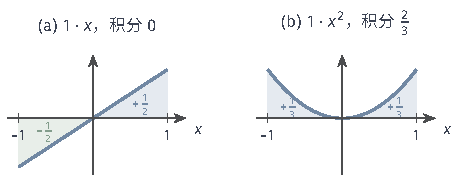
\includegraphics[width=78.2mm]{figures/02-abstract-mathematics/03-function-spaces/tikz/c1-integral-orthogonality/figure.pdf}
  \caption{积分内积下的正交。$[-1,1]$上取Lebesgue测度，曲线是两个函数的乘积，阴影面积带符号累计后即为内积。(a)$1\cdot x$的正负面积各为$\tfrac12$，内积为$0$，$1$与$x$正交；(b)$1\cdot x^2$处处非负，内积为$\tfrac23$，$1$与$x^2$不正交。正交与否只看积分，与曲线的倾角无关。}
  \label{fig:fs-integral-orthogonality}
\end{figure}

\paragraph{复内积的约定}
信号和频域表示需要复值函数。复线性空间上的内积改为共轭对称：$\langle g,f\rangle=\overline{\langle f,g\rangle}$，并且全书统一约定内积对第一个变量共轭线性、对第二个变量线性，即
\[
 \langle af,g\rangle=\bar a\langle f,g\rangle,\qquad \langle f,ag\rangle=a\langle f,g\rangle .
\]
积分内积相应写作$\langle f,g\rangle=\int\overline{f}\,g\,d\mu$。共轭不可省略：在$[-\pi,\pi]$上取$f(x)=e^{ix}$，若不取共轭，$\int f\cdot f\,dx=\int e^{2ix}\,dx=0$，一个非零函数的“长度”会是零；取共轭后$\langle f,f\rangle=\int|e^{ix}|^2\,dx=2\pi$。Cauchy--Schwarz不等式在复情形仍成立（把上面的$t$换成适当的复数），本章主线只用实内积。

\paragraph{范数何时来自内积}
内积诱导的范数满足\term{平行四边形恒等式}（parallelogram identity）
\[
 \|f+g\|^2+\|f-g\|^2=2\|f\|^2+2\|g\|^2,
\]
只需把两边按内积展开，交叉项相互抵消。一般的范数未必满足它。在$C([0,1])$上取最大偏差$\|f\|_\infty=\sup_x|f(x)|$，令$f=1$、$g=x$：$\|f+g\|_\infty=2$，$\|f-g\|_\infty=1$，左边为$5$；$\|f\|_\infty=\|g\|_\infty=1$，右边为$4$。所以最大偏差范数不来自任何内积，$C([0,1])$在这个范数下即使完备，也不是Hilbert空间。“有没有内积”和“是否完备”是两个独立的判断。

\paragraph{有限维直觉的边界}
在有限维空间中，任意两个范数等价，即存在常数$c,C>0$使$c\|v\|_a\leq\|v\|_b\leq C\|v\|_a$，所以范数的选择不影响收敛与完备性。这一结论不能搬到无限维。在$C([0,1])$上，$\|f\|_2\leq\|f\|_\infty$总成立（被积函数不超过$\|f\|_\infty^2$），反方向却没有常数：取$f_n(x)=x^n$，
\[
 \|x^n\|_\infty=1,\qquad \|x^n\|_2=\Bigl(\int_0^1x^{2n}\,dx\Bigr)^{1/2}=\frac{1}{\sqrt{2n+1}}\to0,
\]
比值$\|x^n\|_\infty/\|x^n\|_2=\sqrt{2n+1}$无界。同一个函数集合上的两个范数可以给出完全不同的收敛判断，斜坡例子中的完备性差异也由此而来。

% 第1章第3节：连续函数空间（一致范数与一致收敛；输入域与范数的改变）。

\section{连续函数空间}
\label{sec:fs-continuous}

上一节的定义需要一个完整的例子来落地。本节固定紧区间上的连续函数，配上最大偏差范数，证明得到的是Banach空间。这是最接近一元分析经验的函数空间；随后我们改变输入域和范数，看哪些结论需要重新检查。

\subsection{一致范数与一致收敛}
\label{sec:fs-uniform-norm}

在$C([a,b])$上定义
\begin{equation}
 \|f\|_\infty=\sup_{x\in[a,b]}|f(x)|,
 \label{eq:fs-uniform-norm}
\end{equation}
称为\term{一致范数}（uniform norm）或上确界范数。$|f|$是紧集上的连续函数，由最值定理（定理~\ref{thm:metric-extreme-value}）取到最大值，所以上确界有限，而且实际上是最大值。

范数公理逐条成立。若$\|f\|_\infty=0$，则每一点$|f(x)|\leq0$，$f=0$。齐次性来自$|cf(x)|=|c||f(x)|$在每点成立后取上确界。对三角不等式，每个$x$处都有$|f(x)+g(x)|\leq|f(x)|+|g(x)|\leq\|f\|_\infty+\|g\|_\infty$，右边与$x$无关，对$x$取上确界即得$\|f+g\|_\infty\leq\|f\|_\infty+\|g\|_\infty$。

\paragraph{范数收敛就是一致收敛}
把$\|f_n-f\|_\infty\to0$按定义展开：对每个$\varepsilon>0$存在$N$，使$n\geq N$时$\sup_x|f_n(x)-f(x)|\leq\varepsilon$，即对\emph{所有}$x$同时有$|f_n(x)-f(x)|\leq\varepsilon$。这正是一致收敛：同一个$N$管住全部输入位置。逐点收敛与一致收敛的区别及$x^n$的经典例子，可参考\BookChapterRef{chap:limits-continuity}{卷一“极限与连续”章}。

图~\ref{fig:fs-uniform-tube}给出了几何图像。$\|f_n-f\|_\infty\leq\varepsilon$等价于$f_n$的整条曲线落在以$f$为中心、上下宽$\varepsilon$的带子里，如(a)所示。(b)中的$x^n$在$[0,1)$上逐点趋于$0$，但每条曲线在靠近$x=1$处都会越出零函数周围的带子：$x^4$在$x=0.15^{1/4}\approx0.62$处越出，$x^{12}$推迟到$x=0.15^{1/12}\approx0.85$，越出点随$n$右移，却始终存在。

\begin{figure}[!htb]
  \centering
  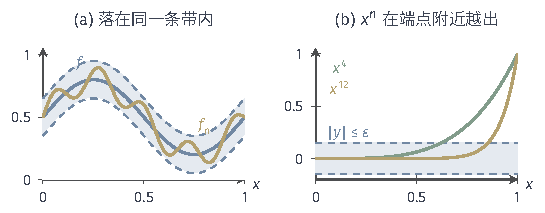
\includegraphics[width=92.2mm]{figures/02-abstract-mathematics/03-function-spaces/tikz/c1-uniform-tube/figure.pdf}
  \caption{一致范数的几何意义。(a)$f(x)=0.5+0.3\sin(2\pi x)$周围宽$\varepsilon=0.15$的带子（浅蓝），$f_n=f+0.1\sin(9\pi x)$整条曲线都在带内，所以$\|f_n-f\|_\infty=0.1\leq\varepsilon$。(b)零函数周围同样宽的带子；$x^4$与$x^{12}$在靠近$x=1$处越出，因为$\|x^n\|_\infty=1$对每个$n$都成立。}
  \label{fig:fs-uniform-tube}
\end{figure}

用一致范数可以把“$x^n$在$[0,1]$上不一致收敛”写成一个具体的数。取$m=2n$，令$t=x^n\in[0,1]$，则
\[
 \|x^n-x^{2n}\|_\infty=\max_{t\in[0,1]}(t-t^2)=\frac14,
\]
最大值在$t=\tfrac12$处取到。这个值不随$n$减小，所以$(x^n)$在$C([0,1])$中连Cauchy列都不是。若把区间缩小到$[0,\tfrac12]$，则$\|x^n\|_\infty=2^{-n}\to0$，一致收敛到零函数。

\paragraph{连续函数空间的完备性}
一致范数下的极限能否留在$C([a,b])$中，是下面这个定理的内容。它的证明包含三个步骤：先构造候选极限，再把逐点收敛加强为一致收敛，最后证明极限连续。三个步骤各有职责，不能从逐点极限直接跳到空间内的收敛。

\begin{theorem}[连续函数空间的完备性]
\label{thm:fs-continuous-complete}
$(C([a,b]),\|\cdot\|_\infty)$是Banach空间。
\end{theorem}

\begin{proof}
设$(f_n)$是一致范数下的Cauchy列。

第一步，逐点构造候选极限。固定$x\in[a,b]$，有$|f_n(x)-f_m(x)|\leq\|f_n-f_m\|_\infty$，所以实数列$(f_n(x))$是Cauchy列。由实数的完备性，它收敛，记极限为$f(x)$。这样得到一个函数$f:[a,b]\to\mathbb R$，但目前只知道$f_n$逐点收敛到它。

第二步，把共同误差界传给极限。给定$\varepsilon>0$，取$N$使$m,n\geq N$时$\|f_n-f_m\|_\infty<\varepsilon$。固定$x$与$n\geq N$，在$|f_n(x)-f_m(x)|<\varepsilon$中令$m\to\infty$，得$|f_n(x)-f(x)|\leq\varepsilon$。这个界与$x$无关，所以$\sup_x|f_n(x)-f(x)|\leq\varepsilon$对所有$n\geq N$成立，即$f_n$一致收敛到$f$。

第三步，证明极限连续。固定$x_0$与$\varepsilon>0$。由第二步取$N$使$\sup_x|f_N(x)-f(x)|<\varepsilon/3$；$f_N$连续，存在$\delta>0$使$|x-x_0|<\delta$时$|f_N(x)-f_N(x_0)|<\varepsilon/3$。对这样的$x$，
\[
 |f(x)-f(x_0)|\leq|f(x)-f_N(x)|+|f_N(x)-f_N(x_0)|+|f_N(x_0)-f(x_0)|<\varepsilon .
\]
所以$f$在$x_0$连续。$x_0$任意，$f\in C([a,b])$；结合第二步，$\|f_n-f\|_\infty\to0$。
\end{proof}

第三步中的“三项误差分解”值得记住：两端的项靠一致收敛统一控制，中间一项靠某个固定的$f_N$的连续性控制。若只有逐点收敛，两端的项无法对邻域内所有$x$同时变小，$x^n$在$[0,1]$上的不连续极限就是例子。

\subsection{输入域与范数的改变}
\label{sec:fs-domain-norm-change}

定理~\ref{thm:fs-continuous-complete}用到了输入域和范数的两项性质：上确界有限，以及一致收敛保持连续。改变输入域或范数时，需要检查的正是这两点。

\paragraph{紧度量空间上的连续函数}
把$[a,b]$换成任意紧度量空间$K$，定义$C(K)$为$K$上的实连续函数，配以$\|f\|_\infty=\sup_{x\in K}|f(x)|$。最值定理在紧度量空间上成立，所以上确界有限；完备性证明的三个步骤只用到实数完备性与度量空间中连续的定义，原样适用。因此$C(K)$也是Banach空间。当$K=\{1,\ldots,n\}$是有限集（任意度量下都紧）时，$C(K)$就是$\mathbb R^n$配最大分量范数。

\paragraph{非紧域与有界连续函数}
在非紧域上，连续函数可能无界：$\mathbb R$上的$f(x)=x$的上确界为$+\infty$，一致“范数”不再是实数。此时改用有界连续函数空间
\[
 C_b(X)=\{f:X\to\mathbb R\ \text{连续}:\ \sup_{x\in X}|f(x)|<\infty\},
\]
配以同样的上确界范数。完备性证明前两步不变。第二步得到的一致误差界还说明极限有界：取定$N$后，对每个$x$都有$|f(x)|\leq\|f_N\|_\infty+\varepsilon$。第三步不依赖紧性。故$C_b(X)$对任意度量空间$X$都是Banach空间。

非紧域上会出现紧区间上没有的现象。在$C_b(\mathbb R)$中取移动的三角形$f_n(x)=\max(0,1-|x-n|)$：每个固定的$x$在$n>|x|+1$后都满足$f_n(x)=0$，所以$f_n$逐点趋于零；但三角形的峰高始终为$1$，$\|f_n\|_\infty=1$，序列不一致收敛。质量没有消失，只是移到了无穷远处。

\paragraph{局部一致收敛}
有些序列在每个有界范围内都一致收敛，在整条实轴上却不收敛。$f_n(x)=x/n$不在$C_b(\mathbb R)$中，但对每个$R>0$，$\sup_{|x|\leq R}|f_n(x)|=R/n\to0$。这种“在每个紧集上一致收敛”称为局部一致收敛，它由一族上确界$\sup_{|x|\leq R}|\cdot|$共同描述，不是单个范数给出的收敛。这类由一族半范数定义的空间不在本章展开；我们只需记住：一致范数关注整个输入域，局部一致收敛只关注每个紧集。

\paragraph{改换范数后的同一集合}
回到同一个集合$C([-1,1])$。在一致范数下它是Banach空间（定理~\ref{thm:fs-continuous-complete}）；换成平方积分范数$\|\cdot\|_2$，第~\ref{sec:fs-banach}小节的斜坡列是Cauchy列却没有连续极限，空间不完备。集合没有变，变的是“接近”的标准。斜坡列在一致范数下不是Cauchy列：对$m>n$，在$x=1/m$处$g_m=1$而$g_n=n/m$，所以$\|g_n-g_m\|_\infty\geq1-n/m$，取$m=2n$即得$\|g_n-g_{2n}\|_\infty\geq\tfrac12$。

平方积分误差关心的是整体偏差，自然的极限是阶跃函数，而它在$0$处的值无关紧要。要让这样的极限有处可去，就需要把成员扩大到可测函数，并且忽略零测集上的差别。这就是下一节积分函数空间的出发点。

% 第1章第4节：积分函数空间（Lp空间与数列空间；Hölder与Minkowski不等式；L∞与本质上界；积分空间的完备性）。

\section{积分函数空间}
\label{sec:fs-integral}

上一节结尾的问题是：平方积分误差下，连续函数的极限可能是阶跃函数这样的不连续函数。本节把误差的累计方式作为出发点，在可测函数的几乎处处等价类上构造两类范数：一类按$p$次幂累计偏差（$1\leq p<\infty$），另一类取忽略零测集后的最大偏差。随后证明三角不等式所需的Hölder与Minkowski不等式，最后证明这些空间都完备。

本节固定测度空间$(X,\mathcal A,\mu)$。可测函数、积分以及单调收敛定理、Fatou引理、控制收敛定理的条件见第~\ref{sec:measure-general-structure}节。

\subsection{$L^p$空间与数列空间}
\label{sec:fs-lp}

\begin{definition}[$L^p$空间]
\label{def:fs-lp}
设$1\leq p<\infty$。若可测函数$f:X\to\mathbb R$满足$\int_X|f|^p\,d\mu<\infty$，称$f$是$p$次可积的。$p$次可积函数的几乎处处等价类全体记为$L^p(\mu)$，并定义
\[
 \bigl\|[f]_\mu\bigr\|_{L^p}=\Bigl(\int_X|f|^p\,d\mu\Bigr)^{1/p}.
\]
当$X$是欧氏空间的子集$\Omega$且$\mu$为Lebesgue测度时，记作$L^p(\Omega)$。
\end{definition}

这个定义需要检查两件事。其一，数值不依赖代表：若$f\sim_\mu g$，则$|f|^p$与$|g|^p$几乎处处相等，零测集上的改动不影响积分，所以两个积分相同。其二，成员对加法封闭。函数$t\mapsto t^p$在$[0,\infty)$上凸（$p\geq1$），所以对$a,b\geq0$有$\bigl(\tfrac{a+b}{2}\bigr)^p\leq\tfrac{a^p+b^p}{2}$，即$(a+b)^p\leq2^{p-1}(a^p+b^p)$。取$a=|f(x)|$、$b=|g(x)|$并积分，
\[
 \int_X|f+g|^p\,d\mu\leq2^{p-1}\Bigl(\int_X|f|^p\,d\mu+\int_X|g|^p\,d\mu\Bigr)<\infty .
\]
数乘的封闭性是显然的，所以$L^p(\mu)$是线性空间。$\|\cdot\|_{L^p}$满足正定性：$\int|f|^p\,d\mu=0$当且仅当$f=0$几乎处处，即$[f]_\mu$是零元素。齐次性直接成立。三角不等式不那么显然，留到第~\ref{sec:fs-holder-minkowski}小节证明。下文在不引起混淆时，用代表$f$代写等价类$[f]_\mu$，并把范数简记为$\|f\|_p$。

\paragraph{不同的$p$衡量不同的整体误差}
$p$越大，局部的大偏差占的比重越大。在$[0,1]$上取窄而高的误差$h=10\cdot\mathbf 1_{[0,0.01]}$：$\|h\|_1=10\times0.01=0.1$，而$\|h\|_2=(100\times0.01)^{1/2}=1$。按绝对偏差累计，这个误差很小；按平方累计，它与“处处偏差为$1$”一样大。选择$p$就是选择怎样为大偏差计价。

用$x^n$可以对照积分误差与最大偏差。在$[0,1]$上，
\[
 \|x^n\|_p=\Bigl(\int_0^1x^{np}\,dx\Bigr)^{1/p}=(np+1)^{-1/p}.
\]
例如$n=10$时，$\|x^{10}\|_1=\tfrac1{11}\approx0.091$，$\|x^{10}\|_2=\tfrac1{\sqrt{21}}\approx0.218$，而$\|x^{10}\|_\infty=1$。图~\ref{fig:fs-xn-norms}(b)画出了三种范数随$n$的变化：两个积分范数都趋于零，$p=2$比$p=1$慢，最大偏差则一直是$1$。原因可以从(a)看出：$x^n$只在越来越窄的一段区间上取大值，积分看到的是这段区间的面积，最大偏差看到的是峰顶。

\begin{figure}[!htb]
  \centering
  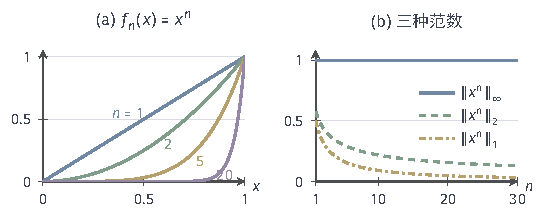
\includegraphics[width=92.3mm]{figures/02-abstract-mathematics/03-function-spaces/tikz/c1-xn-norms/figure.pdf}
  \caption{$x^n$在$[0,1]$上的三种大小。(a)$n=1,2,5,20$时的曲线，函数值集中到右端越来越窄的区间上。(b)三种范数随$n$的变化：$\|x^n\|_\infty=1$，$\|x^n\|_2=(2n+1)^{-1/2}$，$\|x^n\|_1=(n+1)^{-1}$，两个积分范数趋于零，$p=1$下降更快。}
  \label{fig:fs-xn-norms}
\end{figure}

\paragraph{数列空间}
取$X=\mathbb N_+=\{1,2,\ldots\}$与计数测度（每个点的质量为$1$），可测函数就是实数列$x=(x_k)_{k\geq1}$，积分就是求和。此时只有空集是零测集，等价类就是数列本身。$L^p$空间成为
\[
 \ell^p=\Bigl\{x:\ \sum_{k\geq1}|x_k|^p<\infty\Bigr\},\qquad \|x\|_p=\Bigl(\sum_{k\geq1}|x_k|^p\Bigr)^{1/p}.
\]
有限维向量$(x_1,\ldots,x_n)$可以看作后面全为零的数列，$\|x\|_p$就是熟悉的$p$范数，所以$\ell^p$是有限维$p$范数向无限维的自然延伸。数列$x_k=1/k$在$\ell^2$中，因为$\sum_k1/k^2=\pi^2/6$；它不在$\ell^1$中，因为调和级数发散。

\paragraph{平均收敛作为范数收敛}
取概率测度$\mathbb P$，随机变量$Y$的$p$次可积条件就是$\mathbb E|Y|^p<\infty$，范数为$\|Y\|_{L^p(\mathbb P)}=(\mathbb E|Y|^p)^{1/p}$。随机变量的$p$阶平均收敛$\mathbb E|Y_n-Y|^p\to0$因此就是$L^p(\mathbb P)$中的范数收敛。以样本均值为例：设$Y_1,Y_2,\ldots$独立同分布，均值为$m$、方差为$\sigma^2$，则$\bar Y_n=\tfrac1n\sum_{k\leq n}Y_k$满足$\mathbb E(\bar Y_n-m)^2=\sigma^2/n$，即$\|\bar Y_n-m\|_{L^2(\mathbb P)}=\sigma/\sqrt n\to0$。这里只是把已有的平均收敛放进空间结构中，概率收敛的系统理论属于第~\ref{part:probability-spaces}部分，初等的期望与方差计算可参考\BookChapterRef{chap:random-variables}{卷一“随机变量与概率分布”章}。

\subsection{Hölder与Minkowski不等式}
\label{sec:fs-holder-minkowski}

要证明$\|\cdot\|_p$满足三角不等式，需要先控制乘积的积分。设$1<p<\infty$，取$q$满足$\tfrac1p+\tfrac1q=1$，即$q=p/(p-1)$，称$p,q$为\term{共轭指数}（conjugate exponents）。$p=2$时$q=2$；$p=3$时$q=\tfrac32$。

\begin{lemma}[Young不等式]
\label{lem:fs-young}
设$1<p<\infty$，$q$为其共轭指数。对任意$a,b\geq0$，
\[
 ab\leq\frac{a^p}{p}+\frac{b^q}{q},
\]
等号当且仅当$a^p=b^q$。
\end{lemma}

\begin{proof}
固定$b\geq0$，考察$F(s)=\tfrac{s^p}{p}-bs$，$s\geq0$。$F'(s)=s^{p-1}-b$在$s_*=b^{1/(p-1)}$处为零，$s<s_*$时为负、$s>s_*$时为正，所以$F$在$s_*$处取最小值。由$p/(p-1)=q$得$s_*^p=b^q$，于是
\[
 F(s_*)=\frac{b^q}{p}-b\cdot b^{q/p}=\frac{b^q}{p}-b^q=-\frac{b^q}{q},
\]
其中用了$1+q/p=q$。所以$F(a)\geq-b^q/q$，移项即得不等式；等号当且仅当$a=s_*$，即$a^p=b^q$。
\end{proof}

这个不等式有一幅面积图像。共轭条件等价于$(p-1)(q-1)=1$，所以曲线$s=t^{p-1}$也可以写成$t=s^{q-1}$。图~\ref{fig:fs-young-area}中，曲线下方从$0$到$a$的面积是$\int_0^at^{p-1}\,dt=a^p/p$（蓝色），曲线左方从$0$到$b$的面积是$\int_0^bs^{q-1}\,ds=b^q/q$（绿色）。两块区域合起来盖住了矩形$[0,a]\times[0,b]$，所以面积之和不小于$ab$；只有当曲线恰好穿过矩形的右上角，即$b=a^{p-1}$时，两块区域才不多不少地拼成矩形。

\begin{figure}[!htb]
  \centering
  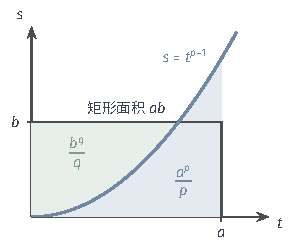
\includegraphics[width=49.6mm]{figures/02-abstract-mathematics/03-function-spaces/tikz/c1-young-area/figure.pdf}
  \caption{Young不等式的面积解释，取$p=3$、$q=\tfrac32$、$a=1$、$b=0.6$。曲线为$s=t^{2}$；蓝色区域面积$a^p/p=\tfrac13$，绿色区域面积$b^q/q\approx0.310$，二者覆盖面积为$ab=0.6$的矩形，多出的部分是曲线在矩形上方的蓝色尖角。}
  \label{fig:fs-young-area}
\end{figure}

\begin{theorem}[Hölder不等式]
\label{thm:fs-holder}
设$1<p<\infty$，$q$为其共轭指数，$f,g$可测。则
\[
 \int_X|fg|\,d\mu\leq\|f\|_p\,\|g\|_q ,
\]
其中右边允许取$+\infty$。特别地，$f\in L^p(\mu)$、$g\in L^q(\mu)$时$fg\in L^1(\mu)$。
\end{theorem}

\begin{proof}
若右边为$+\infty$，无需证明。若$\|f\|_p=0$，则$f=0$几乎处处，$fg=0$几乎处处，左边为零；$\|g\|_q=0$同理。下设$0<\|f\|_p,\|g\|_q<\infty$。在Young不等式中逐点取$a=|f(x)|/\|f\|_p$、$b=|g(x)|/\|g\|_q$，得
\[
 \frac{|f(x)g(x)|}{\|f\|_p\|g\|_q}\leq\frac{|f(x)|^p}{p\|f\|_p^p}+\frac{|g(x)|^q}{q\|g\|_q^q}.
\]
两边积分，右边等于$\tfrac1p+\tfrac1q=1$，再乘以$\|f\|_p\|g\|_q$即得结论。
\end{proof}

归一化这一步的作用是把两个任意大小的函数缩放到“单位大小”，使Young不等式右边的两项积分后恰好凑成$1$。由证明还可以读出等号条件：在每一点都需要$a^p=b^q$，即$|f|^p$与$|g|^q$几乎处处成比例。在$[0,1]$上取$f=x$、$g=x^2$、$p=3$、$q=\tfrac32$：$|f|^p=x^3=|g|^q$，左边$\int_0^1x^3\,dx=\tfrac14$，右边$\|x\|_3\|x^2\|_{3/2}=(\tfrac14)^{1/3}(\tfrac14)^{2/3}=\tfrac14$，等号成立。若取$f=1$、$g=x$、$p=q=2$，左边$\tfrac12$，右边$1\cdot(\tfrac13)^{1/2}\approx0.577$，不等式是严格的。

\begin{theorem}[Minkowski不等式]
\label{thm:fs-minkowski}
设$1\leq p<\infty$，$f,g\in L^p(\mu)$。则$\|f+g\|_p\leq\|f\|_p+\|g\|_p$。因此$(L^p(\mu),\|\cdot\|_p)$是赋范空间。
\end{theorem}

\begin{proof}
$p=1$时，对逐点不等式$|f+g|\leq|f|+|g|$积分即可。设$1<p<\infty$。由第~\ref{sec:fs-lp}小节，$f+g\in L^p$，所以$\int|f+g|^p\,d\mu<\infty$。若它为零，结论平凡，下设它为正。

先把$p$次幂拆成两项：
\[
 |f+g|^p=|f+g|^{p-1}|f+g|\leq|f+g|^{p-1}|f|+|f+g|^{p-1}|g| .
\]
再对每一项用Hölder不等式。由$(p-1)q=p$，$|f+g|^{p-1}$的$q$次积分为$\int|f+g|^p\,d\mu$，所以
\[
 \int|f+g|^{p-1}|f|\,d\mu\leq\Bigl(\int|f+g|^p\,d\mu\Bigr)^{1/q}\|f\|_p ,
\]
第二项同理。两式相加，
\[
 \int|f+g|^p\,d\mu\leq\Bigl(\int|f+g|^p\,d\mu\Bigr)^{1/q}\bigl(\|f\|_p+\|g\|_p\bigr).
\]
左右同除以$(\int|f+g|^p\,d\mu)^{1/q}$（它有限且为正），由$1-\tfrac1q=\tfrac1p$得$\|f+g\|_p\leq\|f\|_p+\|g\|_p$。
\end{proof}

证明中两处条件都不能省：除法要求$\int|f+g|^p\,d\mu$有限且为正，前者来自第~\ref{sec:fs-lp}小节的封闭性估计，后者单独处理。

\paragraph{$0<p<1$时三角不等式失效}
公式$(\int|f|^p\,d\mu)^{1/p}$对$0<p<1$也能计算，但它不是范数。取两点集$\{1,2\}$上的计数测度，$x=(1,0)$、$y=(0,1)$，则$\|x\|_p=\|y\|_p=1$，而
\[
 \|x+y\|_p=(1^p+1^p)^{1/p}=2^{1/p}>2=\|x\|_p+\|y\|_p .
\]
$p=\tfrac12$时左边等于$4$。几何上，范数的单位球$\{v:\|v\|\leq1\}$必定是凸集：若$\|u\|,\|v\|\leq1$，则$\|tu+(1-t)v\|\leq t\|u\|+(1-t)\|v\|\leq1$。图~\ref{fig:fs-unit-balls}画出了平面上$\{|x_1|^p+|x_2|^p\leq1\}$的边界：$p=1,2,\infty$时分别是菱形、圆和正方形，都是凸的；$p=\tfrac12$时边界向内凹，$(1,0)$与$(0,1)$的中点$(\tfrac12,\tfrac12)$满足$2(\tfrac12)^{1/2}\approx1.41>1$，落在集合之外。这正是三角不等式失效的几何表现。

\begin{figure}[!htb]
  \centering
  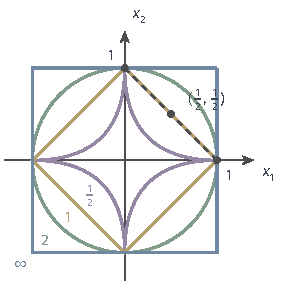
\includegraphics[width=48.6mm]{figures/02-abstract-mathematics/03-function-spaces/tikz/c1-unit-balls/figure.pdf}
  \caption{平面上集合$\{|x_1|^p+|x_2|^p\leq1\}$的边界，曲线旁的数字为$p$；$p=\infty$时为$\max(|x_1|,|x_2|)\leq1$。$p\geq1$时集合是凸的；$p=\tfrac12$时边界内凹，$(1,0)$与$(0,1)$连线的中点$(\tfrac12,\tfrac12)$落在集合外，对应的公式不满足三角不等式。}
  \label{fig:fs-unit-balls}
\end{figure}

\paragraph{$L^2$上的内积}
$p=2$时共轭指数也是$2$，Hölder不等式说明$\int|fg|\,d\mu\leq\|f\|_2\|g\|_2<\infty$，所以
\[
 \langle f,g\rangle=\int_Xfg\,d\mu,\qquad f,g\in L^2(\mu)
\]
有定义，且不依赖代表。对称性与线性来自积分的性质，正定性来自“$\int f^2\,d\mu=0$当且仅当$f=0$几乎处处”。它诱导的范数正是$\|\cdot\|_2$。因此$L^2(\mu)$是内积空间；等第~\ref{sec:fs-lp-completeness}小节证明完备性后，它就是Hilbert空间。

\subsection{$L^\infty$与本质上界}
\label{sec:fs-linfty}

最大偏差也要适应“忽略零测集”的约定。普通上确界会被单个点的值左右，而等价类中的代表可以在零测集上任意改值，所以需要一个只看“几乎处处”的上界。

\begin{definition}[本质上确界与$L^\infty$]
\label{def:fs-linfty}
对可测函数$f$，定义
\[
 \|f\|_\infty=\inf\{M\geq0:\ |f|\leq M\ \text{在}\ \mu\ \text{下几乎处处成立}\},
\]
称为$|f|$的\term{本质上确界}（essential supremum），约定空集的下确界为$+\infty$。本质上确界有限的可测函数称为本质有界的；其几乎处处等价类全体记为$L^\infty(\mu)$。
\end{definition}

先看下确界能否取到。记$M_0=\|f\|_\infty<\infty$，对每个正整数$k$，集合$\{|f|>M_0+1/k\}$是零测集；它们的并$\{|f|>M_0\}$是可数个零测集之并，仍为零测集。所以$|f|\leq\|f\|_\infty$几乎处处成立，下确界是可以达到的。由此也看出数值不依赖代表：若$g\sim_\mu f$，则$\{|g|>M\}\subseteq\{|f|>M\}\cup\{f\neq g\}$，两类函数的本质上界相同。

本质上确界与普通上确界可以相差很远。在$[0,1]$上取Lebesgue测度，令$f(x)=x$，但把$f(\tfrac12)$改为$2$。普通上确界是$2$，而$|f|\leq1$只在单点$\{\tfrac12\}$外成立，所以本质上确界是$1$，如图~\ref{fig:fs-essential-sup}所示。更极端地，有理点示性函数$\mathbf 1_{\mathbb Q\cap[0,1]}$的普通上确界是$1$，本质上确界是$0$，因为有理点只有可数个，组成零测集。这也说明：$\|f\|_\infty\leq M$只保证某个零测集之外处处$|f|\leq M$，并不保证类中任意一个代表在每一点都受这个界控制。若$f$在区间上连续，则$\{|f|>M\}$是开集，非空即有正测度，所以连续函数的本质上确界等于普通上确界。

\begin{figure}[!htb]
  \centering
  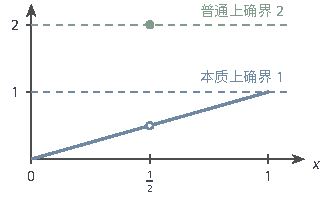
\includegraphics[width=56.1mm]{figures/02-abstract-mathematics/03-function-spaces/tikz/c1-essential-sup/figure.pdf}
  \caption{本质上确界忽略零测集。$[0,1]$上取Lebesgue测度，$f(x)=x$，只把$f(\tfrac12)$改为$2$（绿点，空心圈为原值）。普通上确界被这一个点抬到$2$；单点测度为零，本质上确界仍为$1$。}
  \label{fig:fs-essential-sup}
\end{figure}

\paragraph{范数公理与积分配对}
$\|\cdot\|_\infty$在$L^\infty(\mu)$上是范数，论证的关键是把例外集合并成一个零测集。正定性：若$\|f\|_\infty=0$，由上一段$|f|\leq0$几乎处处，即$f=0$几乎处处。齐次性由$|cf|=|c||f|$得到。三角不等式：$|f|\leq\|f\|_\infty$在零测集$N_f$外成立，$|g|\leq\|g\|_\infty$在零测集$N_g$外成立，于是在$N_f\cup N_g$之外$|f+g|\leq\|f\|_\infty+\|g\|_\infty$，例外集仍是零测集。

$L^\infty$与$L^1$之间有一个自然的积分配对，它是Hölder不等式在端点$p=1$、$q=\infty$的形式：由$|fg|\leq|f|\,\|g\|_\infty$几乎处处成立并积分，
\[
 \int_X|fg|\,d\mu\leq\|f\|_1\,\|g\|_\infty .
\]
约定$\tfrac1\infty=0$后，Hölder不等式对所有共轭指数对$1\leq p\leq\infty$都成立。第~\ref{sec:lfo-lp-dual}小节将从这个配对出发研究$L^p$上的线性泛函。

\paragraph{有界数列空间}
取$\mathbb N_+$上的计数测度，只有空集零测，本质上确界就是普通上确界，得到有界数列空间$\ell^\infty=\{x:\sup_k|x_k|<\infty\}$。常数列$(1,1,1,\ldots)$在$\ell^\infty$中，却不在任何$\ell^p$（$p<\infty$）中。第~\ref{sec:fs-density-separability}小节将看到，$\ell^\infty$与$L^\infty([0,1])$都“太大”，无法用可数个元素逼近；第~\ref{sec:lfo-weak-star}小节则会在$L^\infty$上使用另一种更弱的收敛。

\subsection{积分空间的完备性}
\label{sec:fs-lp-completeness}

现在回答本节开头的问题：积分误差下的Cauchy列是否一定有极限？下面的定理对所有$1\leq p\leq\infty$给出肯定回答，但有限$p$与$p=\infty$的证明方式不同，不能把一个套到另一个上。

\begin{theorem}[积分空间的完备性]
\label{thm:fs-lp-complete}
对任意测度空间与$1\leq p\leq\infty$，$L^p(\mu)$是Banach空间。特别地，$L^2(\mu)$是Hilbert空间。
\end{theorem}

\begin{proof}
先设$1\leq p<\infty$，$(f_n)$是$L^p$中的Cauchy列。证明分五步：抽出快速子列，构造控制函数，定义候选极限，证明子列收敛，最后回到整列。

第一步，抽取相邻差可求和的子列。由Cauchy条件，可以递归地取$n_1<n_2<\cdots$，使$m,n\geq n_k$时$\|f_n-f_m\|_p<2^{-k}$。于是$\|f_{n_{k+1}}-f_{n_k}\|_p<2^{-k}$，$\sum_k\|f_{n_{k+1}}-f_{n_k}\|_p<\infty$。取定各项的可测代表。

第二步，构造控制函数。令
\[
 S_m=|f_{n_1}|+\sum_{k=1}^m|f_{n_{k+1}}-f_{n_k}|,\qquad S=\lim_{m\to\infty}S_m\in[0,\infty].
\]
由Minkowski不等式，$\|S_m\|_p\leq\|f_{n_1}\|_p+\sum_k\|f_{n_{k+1}}-f_{n_k}\|_p=:C<\infty$，界与$m$无关。$S_m^p$逐点单调上升到$S^p$，由单调收敛定理，$\int S^p\,d\mu=\lim_m\int S_m^p\,d\mu\leq C^p$。所以$S\in L^p$，特别地$S<\infty$几乎处处。

第三步，定义候选极限。在$\{S<\infty\}$上，级数$f_{n_1}+\sum_k(f_{n_{k+1}}-f_{n_k})$绝对收敛，其部分和恰为$f_{n_{k+1}}$；令$f$为其和，在零测集$\{S=\infty\}$上令$f=0$。$f$是可测函数列的几乎处处极限，因而可测；$|f|\leq S$，所以$f\in L^p$。至此子列$f_{n_j}\to f$几乎处处。

第四步，证明子列依范数收敛。固定$j$，在$\{S<\infty\}$上$f-f_{n_j}=\lim_{m\to\infty}(f_{n_m}-f_{n_j})$。由Fatou引理与Minkowski不等式，
\[
 \int|f-f_{n_j}|^p\,d\mu\leq\liminf_{m\to\infty}\int|f_{n_m}-f_{n_j}|^p\,d\mu
 \leq\Bigl(\sum_{k\geq j}\|f_{n_{k+1}}-f_{n_k}\|_p\Bigr)^p,
\]
右边是收敛级数的尾和的$p$次方，趋于零。所以$\|f_{n_j}-f\|_p\to0$。

第五步，回到整列。给定$\varepsilon>0$，取$N$使$m,n\geq N$时$\|f_n-f_m\|_p<\varepsilon$，再取$j$使$n_j\geq N$且$\|f_{n_j}-f\|_p<\varepsilon$。则$n\geq N$时$\|f_n-f\|_p\leq\|f_n-f_{n_j}\|_p+\|f_{n_j}-f\|_p<2\varepsilon$。

再设$p=\infty$。取$L^\infty$中的Cauchy列$(f_n)$的代表。对每对$m,n$，$|f_n-f_m|\leq\|f_n-f_m\|_\infty$在某个零测集$E_{m,n}$之外成立。令$E=\bigcup_{m,n}E_{m,n}$，它是可数个零测集之并，仍为零测集。在$X\setminus E$上，所有这些不等式同时成立，所以$(f_n)$在$X\setminus E$上一致Cauchy。与定理~\ref{thm:fs-continuous-complete}的前两步相同，$f_n$在$X\setminus E$上一致收敛到某个函数$f$；在$E$上令$f=0$。$f$是可测函数列在$X\setminus E$上的逐点极限，因而可测；$\sup_{x\notin E}|f_n(x)-f(x)|\to0$给出$\|f_n-f\|_\infty\to0$。取$n_0$使$\|f_{n_0}-f\|_\infty\leq1$，则$\|f\|_\infty\leq\|f_{n_0}\|_\infty+1<\infty$，所以$f\in L^\infty$。

最后，$L^2$的范数由内积诱导，完备后即为Hilbert空间。
\end{proof}

两种证明的差别值得对照。有限$p$的论证没有一致性可用，只能先抽子列，借$S\in L^p$得到几乎处处收敛，再用Fatou引理把逐点信息转为积分信息；$p=\infty$的论证则把可数个例外集合并成一个零测集，在其补集上做一致收敛，与连续函数空间的证明如出一辙。

证明的前三步还给出了一个单独有用的结论，第~\ref{sec:fs-convergence-modes}小节比较收敛方式时会用到。

\begin{theorem}[范数收敛的几乎处处收敛子列]
\label{thm:fs-ae-subsequence}
设$1\leq p<\infty$，$f_n\to f$在$L^p(\mu)$中成立。则存在子列$(f_{n_k})$使$f_{n_k}\to f$几乎处处成立。
\end{theorem}

\begin{proof}
收敛列是Cauchy列。定理~\ref{thm:fs-lp-complete}证明的前四步构造出子列和函数$\tilde f$，使$f_{n_k}\to\tilde f$几乎处处且在$L^p$中成立。$L^p$极限唯一，所以$\tilde f=f$几乎处处。
\end{proof}

回到斜坡例子。在$L^2([-1,1])$中，$\operatorname{sgn}$的等价类是一个合法元素，并且
\[
 \|g_n-\operatorname{sgn}\|_2^2=2\int_0^{1/n}(1-nx)^2\,dx=\frac{2}{3n}\to0 .
\]
所以在$L^2$中，斜坡列有了极限。$\operatorname{sgn}$在$0$处取什么值无关紧要，这正是取等价类的用意。

% 第1章第5节：空间之间的关系（包含关系与范数比较；换测度后的元素与范数；稠密子集与可分性；收敛方式与误差传递）。

\section{空间之间的关系}
\label{sec:fs-relations}

前两节分别构造了连续函数空间、$L^p$空间和数列空间。同一个函数常常同时属于几个空间，同一个误差也可以在几种范数下计算。本节分四个问题比较它们：成员能否从一个空间转入另一个空间；换一个测度后元素与范数怎样变化；能否用简单的、可数的对象逼近一般成员；以及不同意义下的收敛能互相推出什么。每个问题都先固定比较的对象，再给出足够的条件。

\subsection{包含关系与范数比较}
\label{sec:fs-inclusions}

\paragraph{有限测度下的包含}
在总测度有限的空间上，小范围的大值是影响可积性的主要因素，指数越高越难可积。

\begin{theorem}[有限测度下的$L^p$包含]
\label{thm:fs-lp-inclusion}
设$\mu(X)<\infty$，$1\leq p<q\leq\infty$。则$L^q(\mu)\subseteq L^p(\mu)$，并且对所有$f\in L^q(\mu)$，
\begin{equation}
 \|f\|_p\leq\mu(X)^{1/p-1/q}\,\|f\|_q ,
 \label{eq:fs-lp-inclusion}
\end{equation}
其中$q=\infty$时$1/q=0$。
\end{theorem}

\begin{proof}
设$q<\infty$。对$|f|^p\cdot1$使用Hölder不等式，指数取$r=q/p>1$与其共轭指数$r'=q/(q-p)$：
\[
 \int_X|f|^p\,d\mu\leq\Bigl(\int_X|f|^q\,d\mu\Bigr)^{p/q}\Bigl(\int_X1\,d\mu\Bigr)^{(q-p)/q}=\|f\|_q^p\,\mu(X)^{1-p/q}.
\]
两边开$p$次方即得式~\eqref{eq:fs-lp-inclusion}。$q=\infty$时直接由$|f|^p\leq\|f\|_\infty^p$几乎处处成立并积分，得$\|f\|_p\leq\mu(X)^{1/p}\|f\|_\infty$。
\end{proof}

\paragraph{计数测度下的反向包含}
在计数测度下，情况正好相反：总测度无限，但每个点的质量至少为$1$，不会出现“小范围的大值”，影响可求和性的是尾部衰减的快慢。对$p<q$，$\ell^p\subseteq\ell^q$且$\|x\|_q\leq\|x\|_p$。证明只需归一化：设$\|x\|_p=1$，则每个$|x_k|\leq1$，从而$|x_k|^q\leq|x_k|^p$，求和得$\|x\|_q^q\leq1$；一般情形由齐次性得到。

图~\ref{fig:fs-inclusions}把两种方向放在一起。在$(0,1]$上，$x^{-1/2}$可积但平方不可积（$\int_0^1x^{-1}\,dx$发散），$x^{-1/4}$平方可积但无界；在$\mathbb N_+$上，$(1/k)$平方可和但不可和，常数列有界但不平方可和。包含的方向取决于测度：有限测度下指数大的空间小，计数测度下指数小的空间小。在$\mathbb R$上的Lebesgue测度下，两个方向都不成立：$x^{-1/2}\mathbf 1_{(0,1]}$属于$L^1$而不属于$L^2$，$1/(1+|x|)$属于$L^2$（积分为$2$）而不属于$L^1$。

\begin{figure}[!htb]
  \centering
  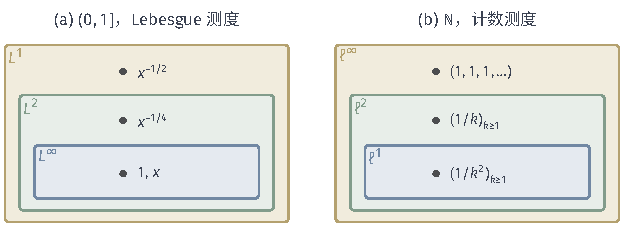
\includegraphics[width=105.7mm]{figures/02-abstract-mathematics/03-function-spaces/tikz/c1-inclusions/figure.pdf}
  \caption{两种测度下的包含方向，嵌套的框表示集合包含，点为各层之间的例子。(a)$(0,1]$上取Lebesgue测度，总质量有限：$L^\infty\subseteq L^2\subseteq L^1$，$x^{-1/4}$在$L^2$中但无界，$x^{-1/2}$可积但不平方可积。(b)$\mathbb N_+$上取计数测度：$\ell^1\subseteq\ell^2\subseteq\ell^\infty$，方向相反。}
  \label{fig:fs-inclusions}
\end{figure}

\paragraph{连续函数进入积分空间}
把一个连续函数“看作”$L^p$中的元素，实际上是一个映射。设$K$是紧度量空间，$\mu$是$K$上的有限Borel测度。连续函数有界且Borel可测，所以$\iota(f)=[f]_\mu$定义了线性映射$\iota:C(K)\to L^p(\mu)$，并且由定理~\ref{thm:fs-lp-inclusion}，
\[
 \|\iota(f)\|_p\leq\mu(K)^{1/p}\|f\|_\infty .
\]
这个映射不一定单射。若$\mu$是全支撑的，即每个非空开集的测度为正，则$f\neq g$时$\{f\neq g\}$是非空开集，测度为正，所以$\iota(f)\neq\iota(g)$。若$\mu$不是全支撑的，例如在$K=[0,1]$上令$\mu(A)$为$A\cap[0,\tfrac12]$的长度，则$f(x)=\max(0,x-\tfrac12)$是非零连续函数，而$\iota(f)=0$。所以只有核实了单射条件，才能把$C(K)$当作$L^p(\mu)$的子空间。

有限测度的假设也不能省。在$\mathbb R$上取Lebesgue测度，常数函数$1$属于$C_b(\mathbb R)$，却不属于任何$L^p$（$p<\infty$）。再取$h_n=\tfrac1n\mathbf 1_{[0,n^2]}$，有$\|h_n\|_\infty=\tfrac1n\to0$，而$\|h_n\|_2^2=\tfrac1{n^2}\cdot n^2=1$：高度在降低，支撑却在扩大，最大偏差趋于零不能推出平方积分误差趋于零。

\subsection{换测度后的元素与范数}
\label{sec:fs-change-of-measure}

同一个可测集合上换一个测度，首先改变的是“哪些差别不计”，其次才是误差的大小。设$\mu,\nu$是同一可测空间上的两个测度。若每个$\mu$零测集也是$\nu$零测集，称$\nu$关于$\mu$\term{绝对连续}（absolutely continuous），记作$\nu\ll\mu$；若两个方向都成立，称它们为\term{等价测度}（equivalent measures）。这些概念见第~\ref{sec:measure-absolute-continuity}节，Radon--Nikodym定理见第~\ref{sec:density-radon-nikodym}节。

\paragraph{零集关系与等价类}
若$\nu\ll\mu$，则$\mu$下几乎处处相等的两个函数在$\nu$下也几乎处处相等，所以$[f]_\mu\mapsto[f]_\nu$不依赖代表，是可测函数等价类之间良定义的线性映射。但它不一定是单射，也不一定保持可积性。

以$[0,1]$上的Lebesgue测度$\mu$与$d\nu=w\,d\mu$为例，其中$w\geq0$可测。由第~\ref{sec:density-weighted-measure}节，$\nu(A)=\int_Aw\,d\mu$是测度且$\nu\ll\mu$，并且$\int h\,d\nu=\int hw\,d\mu$对非负可测$h$成立。若$w=2\cdot\mathbf 1_{[0,1/2]}$，则$f=\mathbf 1_{(1/2,1]}$在$\mu$下不是零元素，在$\nu$下却是：新测度把原来不同的元素合并了。若$w>0$几乎处处，则$\mu\ll\nu$也成立，两个测度识别相同的零差别。

\paragraph{密度界与范数换算}
零集相同还不能保证误差可以互相控制，这需要密度的上下界。对$1\leq p<\infty$与可测函数$h$，
\[
 \|h\|_{L^p(\nu)}^p=\int_X|h|^p\,w\,d\mu .
\]
若$w\leq C$几乎处处，则$\|h\|_{L^p(\nu)}\leq C^{1/p}\|h\|_{L^p(\mu)}$，所以$L^p(\mu)$的成员都在$L^p(\nu)$中，$\mu$下的收敛推出$\nu$下的收敛。若还有$w\geq c>0$几乎处处，则$c^{1/p}\|h\|_{L^p(\mu)}\leq\|h\|_{L^p(\nu)}$，两个空间的成员相同，范数等价。

没有正下界时，反方向可能失败。取$w(x)=2x$与$f(x)=x^{-1/2}$，则
\[
 \int_0^1|f|^2\,d\mu=\int_0^1\frac{dx}{x}=\infty,\qquad \int_0^1|f|^2\,d\nu=\int_0^1\frac{1}{x}\cdot2x\,dx=2 .
\]
图~\ref{fig:fs-change-of-measure}显示了原因：$|f|^2=1/x$在$0$附近的面积无界，而权重$w=2x$恰好在那里趋于零，乘积是常数$2$。所以$f\in L^2(\nu)$但$f\notin L^2(\mu)$，尽管两个测度的零集相同。这里的$w\leq2$只给出$\|h\|_{L^2(\nu)}\leq\sqrt2\|h\|_{L^2(\mu)}$这一个方向。

\begin{figure}[!htb]
  \centering
  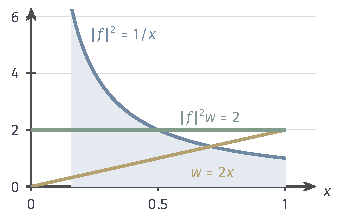
\includegraphics[width=58.1mm]{figures/02-abstract-mathematics/03-function-spaces/tikz/c1-change-of-measure/figure.pdf}
  \caption{换测度后的平方积分。$(0,1]$上$f(x)=x^{-1/2}$，$|f|^2=1/x$（蓝），其下方面积在$0$附近无界（阴影只画到$x=0.16$）；密度$w=2x$（黄）在$0$处趋于零，乘积$|f|^2w=2$（绿）的积分为$2$。所以$f\in L^2(w\,dx)$而$f\notin L^2(dx)$。}
  \label{fig:fs-change-of-measure}
\end{figure}

\paragraph{本质上界的换测度}
$L^\infty$只依赖零集，不需要密度界。若$\nu\ll\mu$，则$\{|f|>M\}$为$\mu$零测时也为$\nu$零测，所以$\|f\|_{L^\infty(\nu)}\leq\|f\|_{L^\infty(\mu)}$；若两个测度等价，本质上确界相同。把有限$p$的估计$C^{1/p}$令$p\to\infty$也能猜出这个结论，但它的成立靠的是零集关系，不是积分公式的极限。

\subsection{稠密子集与可分性}
\label{sec:fs-density-separability}

一般的$L^p$成员可能很不规则，计算和证明时常希望先对简单的函数验证，再推广到全空间。这要求简单函数能以任意精度逼近一般成员。度量空间中，若$D$的闭包是整个空间，称$D$\term{稠密}（dense）（定义~\ref{def:metric-separable}）。

\paragraph{简单函数的稠密性}
取值只有有限多个的可测函数称为简单函数。下面的定理说明，有限$p$的$L^p$中，支撑测度有限的简单函数已经足够。

\begin{theorem}[简单函数在$L^p$中稠密]
\label{thm:fs-simple-dense}
设$1\leq p<\infty$。形如$s=\sum_{i=1}^ka_i\mathbf 1_{A_i}$、其中$\mu(A_i)<\infty$的简单函数在$L^p(\mu)$中稠密。
\end{theorem}

\begin{proof}
先设$f\geq0$。取标准的二进逼近$s_n=\min\bigl(n,\,2^{-n}\lfloor2^nf\rfloor\bigr)$，它是简单函数，满足$0\leq s_n\leq f$且$s_n\uparrow f$逐点成立。于是$|f-s_n|^p\leq f^p$，后者可积，由控制收敛定理$\|f-s_n\|_p\to0$。每个$s_n$的非零取值至少为$2^{-n}$，而$\mu(\{s_n\geq2^{-n}\})\leq\mu(\{f\geq2^{-n}\})\leq2^{np}\|f\|_p^p<\infty$（最后一步是Chebyshev不等式），所以$s_n$的支撑测度有限。一般的$f$写成$f=f^+-f^-$，分别逼近后相减，由三角不等式即得。
\end{proof}

图~\ref{fig:fs-step-density}画出了$f(x)=\sin(\pi x)$的二进逼近。层高每减半一次，阶梯就更贴近曲线：$0\leq f-s_n<2^{-n}$，$n=2$时$L^2$误差约为$0.164$，$n=3$时约为$0.079$。这里$f$有界，所以截断$\min(n,\cdot)$不起作用；对无界的$f$，截断保证每个$s_n$只取有限多个值。

\begin{figure}[!htb]
  \centering
  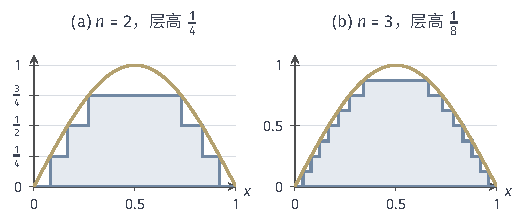
\includegraphics[width=88.7mm]{figures/02-abstract-mathematics/03-function-spaces/tikz/c1-step-density/figure.pdf}
  \caption{用二进简单函数逼近$f(x)=\sin(\pi x)$。$s_n=2^{-n}\lfloor2^nf\rfloor$在$f$落入$[k2^{-n},(k+1)2^{-n})$的位置取值$k2^{-n}$；(a)$n=2$，(b)$n=3$。逐点误差小于$2^{-n}$，$L^2([0,1])$误差约为$0.164$与$0.079$。}
  \label{fig:fs-step-density}
\end{figure}

\paragraph{连续紧支撑函数的稠密性}
在欧氏空间上，还可以用连续函数逼近。记$C_c(\Omega)$为开集$\Omega\subseteq\mathbb R^d$上支撑为紧集的连续函数。

\begin{theorem}[连续紧支撑函数在$L^p(\Omega)$中稠密]
\label{thm:fs-cc-dense}
设$\Omega\subseteq\mathbb R^d$为开集，取Lebesgue测度，$1\leq p<\infty$。则$C_c(\Omega)$在$L^p(\Omega)$中稠密。
\end{theorem}

\begin{proof}
由定理~\ref{thm:fs-simple-dense}和三角不等式，只需逼近有限测度可测集$A\subseteq\Omega$的示性函数。由Lebesgue测度的正则性，对$\varepsilon>0$存在紧集$K$与开集$U$，使$K\subseteq A\subseteq U\subseteq\Omega$且$\lambda(U\setminus K)<\varepsilon$；缩小$U$还可使其闭包是$\Omega$中的紧集。令
\[
 \varphi(x)=\frac{\operatorname{dist}(x,U^c)}{\operatorname{dist}(x,U^c)+\operatorname{dist}(x,K)} .
\]
分母处处为正，$\varphi$连续，在$K$上等于$1$、在$U$外等于$0$、取值在$[0,1]$中，所以$\varphi\in C_c(\Omega)$。$\mathbf 1_A-\varphi$只在$U\setminus K$上非零且绝对值不超过$1$，故$\|\mathbf 1_A-\varphi\|_p^p\leq\lambda(U\setminus K)<\varepsilon$。
\end{proof}

取$\Omega=\mathbb R^d$，定理~\ref{thm:fs-cc-dense}特别给出：$C_c(\mathbb R^d)$在$L^p(\mathbb R^d)$（$1\leq p<\infty$）中稠密。

同样的“先逼近示性函数、再用距离函数构造连续过渡”的论证不依赖欧氏结构，只需测度能被闭集和开集从内外逼近。度量空间上的有限Borel测度具有这种正则性：对每个Borel集$A$与$\varepsilon>0$，存在闭集$F$与开集$U$，使$F\subseteq A\subseteq U$且$\mu(U\setminus F)<\varepsilon$。由此得到紧度量空间上的版本。

\begin{theorem}[紧度量空间上连续函数的稠密性]
\label{thm:fs-continuous-dense-compact}
设$K$为紧度量空间，$\mu$为$K$上的有限Borel测度，$1\leq p<\infty$。则$\{[f]_\mu:f\in C(K)\}$在$L^p(\mu)$中稠密。
\end{theorem}

\begin{proof}
由定理~\ref{thm:fs-simple-dense}，只需逼近Borel集$A$的示性函数。按上面的正则性取闭集$F\subseteq A\subseteq U$（$U$开，$\mu(U\setminus F)<\varepsilon$），定义与定理~\ref{thm:fs-cc-dense}证明中相同的$\varphi$，只把$K$换成$F$。$F$闭、$U^c$闭且二者不交，所以分母处处为正，$\varphi$连续，在$F$上为$1$、在$U$外为$0$，于是$\|\mathbf 1_A-\varphi\|_p^p\leq\mu(U\setminus F)<\varepsilon$。$U=K$或$F=\varnothing$时分别取$\varphi\equiv1$或$\varphi\equiv0$即可。
\end{proof}

\paragraph{区间阶梯函数的稠密性}
在$L^2(0,1)$中，比连续函数更简单的区间阶梯函数也已足够。所谓区间阶梯函数，是有限个区间示性函数的线性组合。给定$f\in L^2(0,1)$与$\varepsilon>0$，由定理~\ref{thm:fs-cc-dense}取连续函数$g$使$\|f-g\|_2<\varepsilon$；$g$在$[0,1]$上一致连续（定理~\ref{thm:metric-compact-uniform}），取$m$足够大，使每个长为$1/m$的区间上$g$的振幅小于$\varepsilon$，令$s$在$[(j-1)/m,j/m)$上取常数$g(j/m)$，则$\|g-s\|_\infty\leq\varepsilon$，从而$\|g-s\|_2\leq\varepsilon$。合起来$\|f-s\|_2<2\varepsilon$。所以区间阶梯函数在$L^2(0,1)$中稠密；同样的论证对任意有限$p$成立。

这些结论回答了斜坡例子留下的问题。$C([-1,1])$在$L^2([-1,1])$中稠密，而$L^2([-1,1])$完备，所以$L^2([-1,1])$正是$(C([-1,1]),\|\cdot\|_2)$的完备化：第~\ref{sec:fs-banach}小节抽象构造出来的“新元素”，在这里被识别为平方可积函数的等价类。用光滑函数逼近需要卷积平滑，留到第~\ref{sec:sob-mollification}小节。

\paragraph{可分性}
稠密子集可以很大。若一个空间有可数的稠密子集，称它\term{可分}（separable）（定义~\ref{def:metric-separable}）。可分空间中的每个元素都能用可数多个“标准对象”中的某些去逼近，这在构造可数正交基、对角线抽取子列时都要用到。

$C([a,b])$可分。Weierstrass逼近定理断言多项式在$(C([a,b]),\|\cdot\|_\infty)$中稠密，证明见第~\ref{sec:apx-polynomial}小节；把多项式的系数换成有理数，误差可以任意小，而有理系数多项式只有可数多个。$\ell^p$（$1\leq p<\infty$）可分：只有有限个非零项且各项为有理数的数列可数，截断尾部和把各项换成有理数都只产生任意小的误差。$L^p(\Omega)$（$1\leq p<\infty$）也可分：由定理~\ref{thm:fs-cc-dense}，可以先用连续紧支撑函数逼近，再在其支撑上用有理系数多项式一致逼近，并乘以有理顶点方体的示性函数（其细节与上面的证明类似，这里从略）。

可数稠密子集与有限维基是两回事。$C([a,b])$中的有理系数多项式可数且稠密，但$e^x$不是其中任何一个的有限线性组合；可分只说明每个元素是可数集合中元素的极限，不说明它能用有限多个方向精确表示。

可分性也不是所有函数空间的共同性质。在$L^\infty([0,1])$中取$f_t=\mathbf 1_{[0,t]}$，$t\in[0,1]$。对$s<t$，$f_t-f_s=\mathbf 1_{(s,t]}$在正测度集上等于$1$，所以$\|f_t-f_s\|_\infty=1$。以每个$f_t$为中心、半径$\tfrac12$的开球两两不交，共有不可数个；若$D$稠密，每个球中至少有$D$的一个元素，且这些元素各不相同，所以$D$不可数。故$L^\infty([0,1])$不可分。同样的论证用于$0$--$1$数列，说明$\ell^\infty$不可分。

\subsection{收敛方式与误差传递}
\label{sec:fs-convergence-modes}

函数列可以在多种意义下收敛。本小节先说明怎样用范数不等式把一种收敛传给另一种，再用三个对照序列标出不能推出的边界。

\paragraph{用范数不等式传递收敛}
设同一线性空间上有两个范数，且存在与序号无关的常数$C$，使$\|h\|_A\leq C\|h\|_B$对所有$h$成立。对$h=f_n-f$使用这个不等式，$\|f_n-f\|_B\to0$即推出$\|f_n-f\|_A\to0$。若两个方向都有这样的常数，两种收敛等价。关键在于常数不随$n$变化，并且两个范数作用于同一列函数、同一个候选极限。

由定理~\ref{thm:fs-lp-inclusion}，在有限测度空间上，$L^q$收敛推出$L^p$收敛（$p<q$），一致收敛推出每个$L^p$收敛。$\mathbb R$上$h_n=\tfrac1n\mathbf 1_{[0,n^2]}$的例子说明，测度无限时后一结论失效。

\paragraph{三个对照序列}
图~\ref{fig:fs-convergence-modes}和表~\ref{tab:fs-convergence-modes}对照了$[0,1]$上Lebesgue测度下的三个序列。

\begin{figure}[!htb]
  \centering
  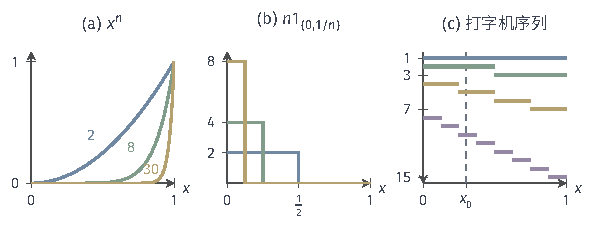
\includegraphics[width=100.4mm]{figures/02-abstract-mathematics/03-function-spaces/tikz/c1-convergence-modes/figure.pdf}
  \caption{三种收敛方式的反例。(a)$x^n$，$n=2,8,30$：逐点趋于端点处为$1$、其余为$0$的函数，$L^p$范数趋于零，最大偏差恒为$1$。(b)窄尖峰$n\mathbf 1_{(0,1/n)}$，$n=2,4,8$：每一点最终为零，积分却恒为$1$。(c)打字机序列的前$15$项，第$k$层把$[0,1)$等分为$2^k$段，依次取各段的示性函数；纵轴为项号，横条为支撑。竖虚线$x=x_0$在每一层恰好穿过一个横条。}
  \label{fig:fs-convergence-modes}
\end{figure}

\begin{table}[!htb]
  \centering
  \begin{tabular}{@{}lccc@{}}
    \toprule
    序列 & 逐点收敛到$0$ & $L^1$收敛到$0$ & 一致收敛到$0$ \\
    \midrule
    $x^n$ & 除$x=1$外 & 是 & 否 \\
    $n\mathbf 1_{(0,1/n)}$ & 是（处处） & 否 & 否 \\
    打字机序列 & 处处不收敛 & 是 & 否 \\
    \bottomrule
  \end{tabular}
  \caption{$[0,1]$上Lebesgue测度下三个序列的收敛性质。}
  \label{tab:fs-convergence-modes}
\end{table}

$x^n$的计算已在第~\ref{sec:fs-lp}小节完成：$\|x^n\|_p=(np+1)^{-1/p}\to0$，逐点极限在$x=1$处为$1$，但这只是一个零测点，所以作为$L^p$元素，逐点极限与零元素相同，两种说法并不矛盾。最大偏差恒为$1$，不一致收敛。

窄尖峰$g_n=n\mathbf 1_{(0,1/n)}$在每个$x$处最终为零：$x\leq0$时恒为零，$x>0$时只要$n>1/x$就有$g_n(x)=0$。但$\|g_n\|_1=1$，$\|g_n\|_2=\sqrt n\to\infty$。逐点收敛允许不同位置在不同时刻进入误差带，因而管不住越来越窄、越来越高的峰。

\begin{example}[打字机序列]
\label{ex:fs-typewriter}
对$k=0,1,2,\ldots$与$j=0,\ldots,2^k-1$，令$h_{k,j}=\mathbf 1_{[j2^{-k},(j+1)2^{-k})}$，并按$k$从小到大、同一层内按$j$从小到大排成一列：$h_{0,0},h_{1,0},h_{1,1},h_{2,0},\ldots$。第$k$层每一项的范数是$\|h_{k,j}\|_p=2^{-k/p}$，随项号增大趋于零，所以序列在每个$L^p$（$p<\infty$）中收敛到$0$。但对每个$x_0\in[0,1)$，每一层恰好有一项在$x_0$处取$1$，其余项取$0$，所以数列$(h_{k,j}(x_0))$中$0$和$1$都出现无穷多次，在任何一点都不收敛。
\end{example}

\paragraph{子列与控制条件}
打字机序列说明$L^p$收敛推不出整列的逐点收敛，但定理~\ref{thm:fs-ae-subsequence}保证可以抽出几乎处处收敛的子列。这里可以直接写出一个：子列$h_{k,0}=\mathbf 1_{[0,2^{-k})}$对每个$x>0$在$2^{-k}<x$后恒为零，所以它在$(0,1]$上逐点收敛到$0$，例外只有零测点$x=0$。

反方向，从几乎处处收敛推出$L^p$收敛需要附加条件。若$f_n\to f$几乎处处，且存在同一个$G\in L^p$使$|f_n|\leq G$几乎处处对所有$n$成立，则$|f|\leq G$，$|f_n-f|^p\leq2^pG^p$可积，由控制收敛定理$\|f_n-f\|_p\to0$。窄尖峰没有这样的控制函数：$\sup_ng_n(x)$在$x\in[\tfrac1{n+1},\tfrac1n)$上至少为$n$，大于$\tfrac1x-1$，不可积。所以“每项各自可积”不能代替“同一个可积函数控制所有项”。

\paragraph{弱收敛的预告}
还有一种收敛不要求整体误差趋于零。在$L^2(0,2\pi)$中取$u_n(x)=\sin(nx)$，有$\|u_n\|_2^2=\pi$，序列不趋于零。但对任意区间$[a,b]\subseteq[0,2\pi]$，
\[
 \int_0^{2\pi}\sin(nx)\,\mathbf 1_{[a,b]}(x)\,dx=\frac{\cos(na)-\cos(nb)}{n}\to0 :
\]
与每个固定的阶跃函数比较，$u_n$越来越接近零函数。这种“通过每个固定的连续线性读取来判断极限”的收敛称为弱收敛，它需要先建立线性泛函，正式定义见第~\ref{sec:lfo-weak-convergence}小节。它与概率测度的弱收敛（第~\ref{sec:wlim-weak-convergence}节）名字相同，但变化的对象与测试对象都不同，不能互换。

% 第1章第6节：Hilbert空间的正交结构（闭子空间的正交投影；正交系与正交基；正交展开与截断误差）。

\section{Hilbert空间的正交结构}
\label{sec:fs-orthogonal}

本节固定一个Hilbert空间$H$，例如$L^2(\mu)$或$\ell^2$，研究两个几何问题：给定一个子空间，能否从中取出离目标最近的分量；能否用一组两两正交的方向给每个元素写出坐标。有限维中的答案是熟悉的，无限维中的新问题是极限是否存在、是否留在子空间里。下一章将把这里的投影看作有界线性算子，本节只建立几何结论。

\subsection{闭子空间的正交投影}
\label{sec:fs-projection}

设$M\subseteq H$是线性子空间，$f\in H$。我们想找$M$中离$f$最近的元素，即达到
\[
 d(f,M)=\inf_{m\in M}\|f-m\|
\]
的$m$。下确界总存在，问题是它能否被$M$中的某个元素取到、取到的元素是否唯一。

\begin{theorem}[闭子空间上的正交投影]
\label{thm:fs-projection}
设$H$为Hilbert空间，$M\subseteq H$为闭线性子空间。则对每个$f\in H$，存在唯一的$m_*\in M$使$\|f-m_*\|=d(f,M)$；并且对$m\in M$，$\|f-m\|=d(f,M)$当且仅当$f-m$与$M$中每个元素正交。
\end{theorem}

\begin{proof}
记$d=d(f,M)$。证明分四步，前两步得到存在性，后两步得到正交刻画与唯一性。

第一步，极小化序列是Cauchy列。取$m_n\in M$使$\|f-m_n\|^2<d^2+1/n$。对$f-m_j$与$f-m_k$使用平行四边形恒等式，
\[
 \|m_j-m_k\|^2=2\|f-m_j\|^2+2\|f-m_k\|^2-4\Bigl\|f-\frac{m_j+m_k}{2}\Bigr\|^2 .
\]
$M$是线性子空间，中点$\tfrac{m_j+m_k}2$在$M$中，所以最后一项的范数平方至少为$d^2$。于是$\|m_j-m_k\|^2<2/j+2/k$，$(m_n)$是Cauchy列。

第二步，极限存在且留在$M$中。$H$完备，所以$m_n$收敛到某个$m_*\in H$；$M$闭，所以$m_*\in M$。由范数的连续性，$\|f-m_*\|=\lim_n\|f-m_n\|=d$。

第三步，最近点的残差与$M$正交。设$m_*$达到$d$，记$r=f-m_*$。任取$m\in M$与实数$t$，$m_*+tm\in M$，所以
\[
 \|r\|^2\leq\|r-tm\|^2=\|r\|^2-2t\langle r,m\rangle+t^2\|m\|^2 .
\]
即$t^2\|m\|^2-2t\langle r,m\rangle\geq0$对所有实数$t$成立。若$\langle r,m\rangle\neq0$，取符号与之相同的足够小的$t$会使左边为负，矛盾；故$\langle r,m\rangle=0$。复Hilbert空间中把$t$换成$t\langle m,r\rangle$即可得到同样的结论。

第四步，正交的残差给出唯一的最近点。设$m_*\in M$满足$f-m_*\perp M$。对任意$m\in M$，$m_*-m\in M$与$f-m_*$正交，由勾股恒等式
\[
 \|f-m\|^2=\|f-m_*\|^2+\|m_*-m\|^2 ,
\]
所以$\|f-m\|\geq\|f-m_*\|$，等号当且仅当$m=m_*$。结合第三步，达到$d$的元素恰好是使残差正交的元素，且只有一个。
\end{proof}

图~\ref{fig:fs-projection-geometry}是这个定理的示意。完备性和闭性在第二步中分工明确：前者保证极小化序列有极限，后者保证极限没有离开$M$。第一步用到了平行四边形恒等式，所以这个论证依赖内积；在一般的Banach空间中，最近点可能不存在，也可能不唯一。

\begin{figure}[!htb]
  \centering
  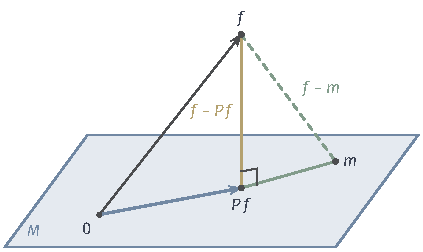
\includegraphics[width=71.7mm]{figures/02-abstract-mathematics/03-function-spaces/tikz/c1-projection-geometry/figure.pdf}
  \caption{闭子空间上的正交投影（示意）。平面代表闭子空间$M$，$Pf$是$M$中离$f$最近的点，残差$f-Pf$与$M$垂直。对$M$中任意另一点$m$，三点构成直角三角形，$\|f-m\|^2=\|f-Pf\|^2+\|Pf-m\|^2$，所以$m$离$f$更远。}
  \label{fig:fs-projection-geometry}
\end{figure}

\paragraph{正交分解与投影的性质}
把定理中的$m_*$记为$P_Mf$，称为$f$在$M$上的\term{正交投影}（orthogonal projection）。记$M^\perp=\{g\in H:\langle g,m\rangle=0\ \text{对所有}\ m\in M\}$为$M$的\term{正交补}（orthogonal complement）。它是闭线性子空间：线性由内积的线性得到，闭性由内积的连续性（Cauchy--Schwarz不等式）得到。定理给出分解
\[
 f=P_Mf+(f-P_Mf),\qquad P_Mf\in M,\quad f-P_Mf\in M^\perp ,
\]
而且这种分解唯一：若$f=m+g=m'+g'$，则$m-m'=g'-g$同时属于$M$与$M^\perp$，与自身正交，只能为零。因此$H=M\oplus M^\perp$。

由正交刻画还可以读出$P_M$的三条性质。线性：$af+bg-(aP_Mf+bP_Mg)=a(f-P_Mf)+b(g-P_Mg)\perp M$，所以$P_M(af+bg)=aP_Mf+bP_Mg$。幂等：$m\in M$时$m$自己就是最近点，$P_M(P_Mf)=P_Mf$。不扩张：由勾股恒等式$\|f\|^2=\|P_Mf\|^2+\|f-P_Mf\|^2$，得$\|P_Mf\|\leq\|f\|$。第~\ref{sec:lfo-self-adjoint}小节将从算子的角度刻画这类映射。

最简单的例子是向常数投影。在$L^2([-1,1])$中取$M=\operatorname{span}\{1\}$，正交条件$\int_{-1}^1(f-c)\,dx=0$给出$c=\tfrac12\int_{-1}^1f\,dx$，即投影是平均值。对$f=x^2$，$P_Mf=\tfrac13$，残差$x^2-\tfrac13$与$1$正交，距离平方为
\[
 \int_{-1}^1\Bigl(x^2-\frac13\Bigr)^2dx=\frac25-\frac49+\frac29=\frac{8}{45} .
\]
这个数在第~\ref{sec:fs-orthonormal-bases}小节的Gram--Schmidt计算中还会出现。

\paragraph{闭性缺失时最近点可能不存在}
定理中的闭性不能去掉。在$H=L^2([-1,1])$中，令$M$为具有连续代表的等价类组成的子空间，它是线性子空间，但由定理~\ref{thm:fs-cc-dense}它在$H$中稠密而不等于$H$，所以不闭。取$f=\operatorname{sgn}$，斜坡给出$\|f-g_n\|_2^2=\tfrac{2}{3n}\to0$，于是$d(f,M)=0$。若下确界被某个$m\in M$取到，则$\|f-m\|_2=0$，$\operatorname{sgn}$与一个连续函数几乎处处相等；而第~\ref{sec:fs-banach}小节已经证明这不可能。所以最近点不存在：每个连续函数都可以再改进，却没有最好的那一个。

本节只处理线性子空间。向一般闭凸集投影时，最近点仍然存在且唯一，但正交条件要换成变分不等式，这与约束优化一起讨论，可参考\BookChapterRef{chap:constrained-optimization}{卷三“有约束优化的求解”章}。

\subsection{正交系与正交基}
\label{sec:fs-orthonormal-bases}

有限维空间中，投影可以用标准正交基的坐标直接写出。现在考察无限多个正交方向。

\begin{definition}[正交归一系]
\label{def:fs-orthonormal}
Hilbert空间$H$中的序列（有限或可数）$(e_j)$称为\term{正交归一系}（orthonormal system），若$\langle e_j,e_k\rangle=\delta_{j,k}$，即两两正交且各自范数为$1$。
\end{definition}

\paragraph{有限个方向上的投影与Bessel不等式}
设$e_1,\ldots,e_m$正交归一，$M_m=\operatorname{span}\{e_1,\ldots,e_m\}$。有限维子空间是闭的（有限维赋范空间完备），所以定理~\ref{thm:fs-projection}适用。记$c_j=\langle e_j,f\rangle$，则
\begin{equation}
 P_{M_m}f=\sum_{j=1}^mc_je_j .
 \label{eq:fs-finite-projection}
\end{equation}
验证只需检查残差：$\langle e_k,f-\sum_jc_je_j\rangle=c_k-c_k=0$对每个$k\leq m$成立，所以残差与$M_m$正交。由勾股恒等式与正交归一性，
\begin{equation}
 \Bigl\|f-\sum_{j=1}^mc_je_j\Bigr\|^2=\|f\|^2-\sum_{j=1}^m|c_j|^2 .
 \label{eq:fs-bessel-error}
\end{equation}

\begin{theorem}[Bessel不等式]
\label{thm:fs-bessel}
设$(e_j)_{j\geq1}$为$H$中的正交归一系，$f\in H$。则$\sum_{j\geq1}|\langle e_j,f\rangle|^2\leq\|f\|^2$。
\end{theorem}

\begin{proof}
由式~\eqref{eq:fs-bessel-error}，左边每个部分和都不超过$\|f\|^2$。非负项级数的部分和有界，级数收敛且和不超过这个界。
\end{proof}

Bessel不等式说明系数平方可和，于是$c_j\to0$：任何元素在越来越靠后的正交方向上的分量都越来越小。

\paragraph{Gram--Schmidt与可数正交基的来源}
正交归一系可以从任意线性无关的序列造出来。设$u_1,u_2,\ldots$线性无关，依次令
\[
 v_k=u_k-\sum_{j<k}\langle e_j,u_k\rangle e_j,\qquad e_k=\frac{v_k}{\|v_k\|} .
\]
$v_k$是$u_k$减去它在$\operatorname{span}\{e_1,\ldots,e_{k-1}\}$上的投影，与之前的方向正交；线性无关保证$v_k\neq0$。归纳可知$\operatorname{span}\{e_1,\ldots,e_k\}=\operatorname{span}\{u_1,\ldots,u_k\}$对每个$k$成立。这就是有限维中的\term{Gram--Schmidt正交化}（Gram--Schmidt orthogonalization），只是现在可以无限地进行下去。

在$L^2([-1,1])$中对$1,x,x^2,x^3$执行这一过程。$e_0=1/\sqrt2$。$x$与$1$正交，$\|x\|^2=\tfrac23$，所以$e_1=\sqrt{3/2}\,x$。对$x^2$，$\langle e_0,x^2\rangle=\tfrac{\sqrt2}3$，$\langle e_1,x^2\rangle=0$，于是$v_2=x^2-\tfrac13$，这正是上一小节向常数投影的残差，$\|v_2\|^2=\tfrac8{45}$，故
\[
 e_2=\sqrt{\tfrac{45}{8}}\Bigl(x^2-\frac13\Bigr)=\sqrt{\tfrac58}\,(3x^2-1).
\]
对$x^3$，它与$e_0,e_2$正交，$\langle e_1,x^3\rangle e_1=\tfrac32\cdot\tfrac25x=\tfrac35x$，于是$v_3=x^3-\tfrac35x$，$\|v_3\|^2=\tfrac27-\tfrac{12}{25}+\tfrac{6}{25}=\tfrac{8}{175}$，故$e_3=\sqrt{7/8}\,(5x^3-3x)$。这些就是归一化的Legendre多项式。图~\ref{fig:fs-legendre-gram-schmidt}对照了正交化前后的函数：(a)中$x^2$与$1$、$x^3$与$x$在大部分区间上走向相近，彼此远不正交；(b)中每个$e_k$恰好比前一个多一次变号。

\begin{figure}[!htb]
  \centering
  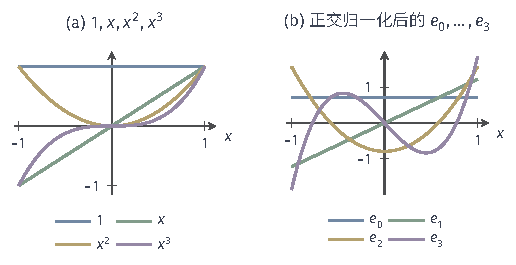
\includegraphics[width=87.3mm]{figures/02-abstract-mathematics/03-function-spaces/tikz/c1-legendre-gram-schmidt/figure.pdf}
  \caption{在$L^2([-1,1])$中对单项式做Gram--Schmidt正交化。(a)$1,x,x^2,x^3$，例如$\langle1,x^2\rangle=\tfrac23\neq0$；(b)得到的$e_0=1/\sqrt2$，$e_1=\sqrt{3/2}\,x$，$e_2=\sqrt{5/8}\,(3x^2-1)$，$e_3=\sqrt{7/8}\,(5x^3-3x)$，两两正交且范数为$1$，$e_k$在$(-1,1)$内恰有$k$个零点。}
  \label{fig:fs-legendre-gram-schmidt}
\end{figure}

同一过程解释了可分Hilbert空间中可数正交归一系的来源。设$H$可分，取可数稠密子集$\{u_k\}$，依次删去能由前面元素线性表出的项，再做Gram--Schmidt，得到正交归一系$(e_j)$，其张成与$\{u_k\}$的张成相同，因而在$H$中稠密。

\paragraph{正交系的完备性}
上面得到的正交系有一个关键性质：它的有限线性组合在$H$中稠密。

\begin{definition}[完备正交系]
\label{def:fs-complete-system}
若正交归一系$(e_j)$的闭线性张成$\overline{\operatorname{span}}\{e_j\}$等于$H$，称它为$H$的\term{完备正交系}（complete orthonormal system），也称\term{标准正交基}（orthonormal basis）。
\end{definition}

这里的“完备”与空间的完备是两个不同的概念：前者说正交系的方向够用，后者说Cauchy列有极限。完备正交系可以用正交性来检验：$(e_j)$完备当且仅当与所有$e_j$都正交的元素只有零。若$(e_j)$完备而$g\perp e_j$对所有$j$成立，则$g$与$\operatorname{span}\{e_j\}$正交，由内积的连续性也与其闭包$H$正交，特别地$\langle g,g\rangle=0$。反之，若闭张成$M\neq H$，取$f\notin M$，由定理~\ref{thm:fs-projection}，$f-P_Mf$是非零元素且与每个$e_j$正交。

\begin{example}[偶方向遗漏奇函数]
\label{ex:fs-even-subspace}
在$L^2([-1,1])$中，偶次的归一化Legendre多项式$e_0,e_2,e_4,\ldots$组成一个无限的正交归一系。但$x$是奇函数，与每个偶函数正交（乘积为奇函数，积分为零），而$x\neq0$，所以这个系不完备。方向有无穷多个，正交性也成立，却仍然遗漏了整个奇函数子空间。

设$E$为几乎处处满足$f(-x)=f(x)$的元素组成的子空间，它是闭的（$L^2$收敛列有几乎处处收敛子列，定理~\ref{thm:fs-ae-subsequence}，极限保持偶性）。任意$f$可以写成$f=\tfrac{f(x)+f(-x)}{2}+\tfrac{f(x)-f(-x)}{2}$，前者是偶函数，后者是奇函数，与$E$正交，所以由定理~\ref{thm:fs-projection}，$P_Ef(x)=\tfrac{f(x)+f(-x)}2$。取$f=e^x$，得$P_Ef=\cosh x$，残差$\sinh x$，见图~\ref{fig:fs-even-odd-projection}；距离平方为$\int_{-1}^1\sinh^2x\,dx=\tfrac{\sinh2}{2}-1\approx0.813$，无论加入多少偶方向都无法减小。
\end{example}

\begin{figure}[!htb]
  \centering
  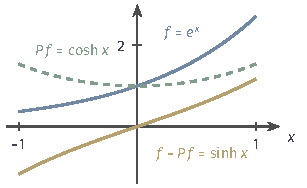
\includegraphics[width=51.9mm]{figures/02-abstract-mathematics/03-function-spaces/tikz/c1-even-odd-projection/figure.pdf}
  \caption{向偶函数子空间的正交投影。$[-1,1]$上$f(x)=e^x$（蓝），投影$Pf=\cosh x$（绿，虚线）为其偶部，残差$f-Pf=\sinh x$（黄）为奇函数，与每个偶函数正交。只用偶方向展开$e^x$时，误差始终至少为$\|\sinh\|_2\approx0.90$。}
  \label{fig:fs-even-odd-projection}
\end{figure}

\subsection{正交展开与截断误差}
\label{sec:fs-orthogonal-expansion}

有了正交归一系，就可以考察无穷级数$\sum_jc_je_j$：它是否收敛，收敛到什么，截断后误差多大。

\begin{theorem}[正交展开与Parseval等式]
\label{thm:fs-parseval}
设$(e_j)_{j\geq1}$为Hilbert空间$H$中的正交归一系，$M=\overline{\operatorname{span}}\{e_j\}$，$f\in H$，$c_j=\langle e_j,f\rangle$。则级数$\sum_jc_je_j$依范数收敛，其和为$P_Mf$。特别地，若$(e_j)$完备，则
\[
 f=\sum_{j=1}^\infty c_je_j\quad(\text{依范数}),\qquad \|f\|^2=\sum_{j=1}^\infty|c_j|^2 .
\]
后一个等式称为\term{Parseval等式}（Parseval identity）。
\end{theorem}

\begin{proof}
记部分和$s_n=\sum_{j\leq n}c_je_j$。对$n>m$，由正交归一性$\|s_n-s_m\|^2=\sum_{m<j\leq n}|c_j|^2$，由Bessel不等式这是收敛级数的一段，所以$(s_n)$是Cauchy列。$H$完备，$s_n$收敛到某个$s$；每个$s_n\in M$而$M$闭，所以$s\in M$。

再验证$f-s\perp M$。对固定的$k$与$n\geq k$，$\langle e_k,f-s_n\rangle=c_k-c_k=0$；令$n\to\infty$，由内积的连续性得$\langle e_k,f-s\rangle=0$。于是$f-s$与$\operatorname{span}\{e_j\}$正交，进而与其闭包$M$正交。由定理~\ref{thm:fs-projection}的正交刻画，$s=P_Mf$。

若$(e_j)$完备，则$M=H$，$P_Mf=f$。在式~\eqref{eq:fs-bessel-error}中令$m\to\infty$，左边趋于$0$，即得Parseval等式。
\end{proof}

对不完备的正交系，展开只恢复$f$在闭张成上的投影，正交补中的分量永远丢失；示例~\ref{ex:fs-even-subspace}中只用偶次Legendre多项式展开$e^x$，奇部$\sinh x$与每个方向都正交，得到的级数和与$e^x$的距离至少为$\|\sinh\|_2$。Bessel不等式与Parseval等式之间的差距，正是这部分丢失的分量。

\paragraph{Legendre多项式的完备性}
判断一个具体的正交系是否完备，需要稠密性论证。对Legendre多项式，三步就够了。由Weierstrass逼近定理，多项式在$(C([-1,1]),\|\cdot\|_\infty)$中稠密；由$\|h\|_2\leq\sqrt2\|h\|_\infty$，一致逼近也是$L^2$逼近；再由定理~\ref{thm:fs-cc-dense}，连续函数在$L^2([-1,1])$中稠密。所以多项式在$L^2([-1,1])$中稠密，而Legendre多项式的张成就是全体多项式，它们组成$L^2([-1,1])$的完备正交系。三角函数系$\{e^{ikx}\}$在$L^2(-\pi,\pi)$中的完备性及傅里叶分析，可参考\BookChapterRef{chap:signal-analysis}{卷三“信号”章}。

\paragraph{截断误差与系数衰减}
固定完备正交系与目标$f$，只改变保留的项数$m$。由式~\eqref{eq:fs-bessel-error}与Parseval等式，
\begin{equation}
 \|f-s_m\|^2=\sum_{j>m}|c_j|^2 ,
 \label{eq:fs-truncation-tail}
\end{equation}
截断误差就是系数平方的尾和。每个$s_m$是$f$在前$m$个方向张成的子空间上的投影，所以在这个子空间内是最好的；但它并没有与其他同样规模的表示比较过，选什么方向是第~\ref{chap:function-approximation}章的问题。

用Legendre多项式展开$\operatorname{sgn}$可以具体看到这些量。$\operatorname{sgn}$是奇函数，只有奇次系数非零；按系数公式精确计算，前几个系数平方为$c_1^2=\tfrac32$，$c_3^2=\tfrac{7}{32}$，$c_5^2=\tfrac{11}{128}$，对应的截断误差$2-\sum_{j\leq m}c_j^2$在$m=1,5,15$时约为$0.500$、$0.195$、$0.077$。图~\ref{fig:fs-legendre-truncation}(a)画出了部分和，(b)把它与$|x|$的展开对照：$|x|$连续，只在$0$处有折角，截断误差下降得快得多，$m=2$时已约为$0.0104$，$m=40$时约为$6\times10^{-6}$；$\operatorname{sgn}$有跳跃，$m=41$时误差仍约为$0.030$。这里只是两个例子的观察；系数衰减与函数光滑性之间的一般关系属于第~\ref{chap:function-approximation}章。

\begin{figure}[!htb]
  \centering
  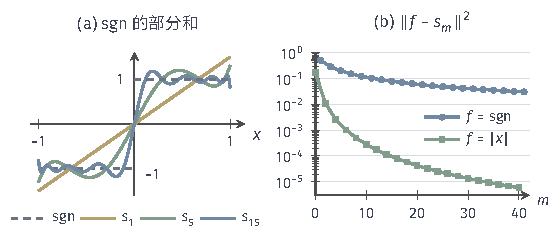
\includegraphics[width=94.9mm]{figures/02-abstract-mathematics/03-function-spaces/tikz/c1-legendre-truncation/figure.pdf}
  \caption{Legendre展开的截断。(a)$\operatorname{sgn}$（虚线）与部分和$s_1,s_5,s_{15}$，其中$s_1=\tfrac32x$；部分和是多项式，在跳跃点附近来回振荡。(b)截断误差$\|f-s_m\|_2^2$（对数纵轴）：$\operatorname{sgn}$取奇数$m$，$|x|$取偶数$m$。两条曲线都单调趋于零，有跳跃的$\operatorname{sgn}$下降慢得多。数值由精确有理运算得到。}
  \label{fig:fs-legendre-truncation}
\end{figure}

\paragraph{从范数收敛到点值收敛}
式~\eqref{eq:fs-truncation-tail}只控制$L^2$误差。图~\ref{fig:fs-legendre-truncation}(a)中的部分和都是连续函数；若它们一致收敛，极限必然连续（定理~\ref{thm:fs-continuous-complete}），而$\operatorname{sgn}$在$0$处跳跃，所以$s_m$不一致收敛到$\operatorname{sgn}$，尽管$L^2$误差趋于零。要从范数收敛得到某点处函数值的收敛，需要“该点的值受范数控制”这样的读取界；$L^2$本身不提供这种界，第~\ref{sec:lfo-point-evaluation}小节将专门讨论这个问题。

% 第1章第7节：本章小结。

\section{本章小结}
\label{sec:fs-summary}

章首的问题是：当表示规模不断变化时，怎样直接比较函数、谈论极限和正交分量。本章的回答可以归结为四个依次进行的选择：选定函数集合，确定什么算作同一个元素，规定误差，检查极限是否留在集合中。

第一个选择决定线性运算是否封闭：连续函数、多项式和固定函数的张成是线性空间，参数化的非线性族一般不是；一维输入也可以产生无限维的函数空间。第二个选择决定元素的身份：用积分衡量误差时，只在零测集上不同的函数必须看成同一个元素，代价是等价类一般没有确定的点值。第三个选择是范数，它让误差满足正定、齐次和三角不等式，从而接入度量空间的全部工具。第四个选择是完备性检查，它同时依赖集合和范数：同一个$C([-1,1])$在一致范数下完备，在平方积分范数下不完备，斜坡逼近阶跃的例子说明了二者的差别，而$L^2([-1,1])$正是后者的完备化。

三类空间的结构可以这样对照。连续函数空间$C(K)$的元素是普通函数，一致范数控制每一点，完备性来自一致收敛保持连续。$L^p(\mu)$的元素是等价类，范数累计整体偏差，Hölder与Minkowski不等式保证范数公理，完备性靠抽子列与Fatou引理（有限$p$）或合并零测例外集（$p=\infty$）得到。数列空间$\ell^p$是计数测度下的$L^p$，等价类退化为数列本身。比较这些空间时，要分清三种保证：同一个函数集合不保证相同的收敛；相同的零集保证换测度后元素的识别一致，却不保证范数可比；只有与序号无关的范数不等式才能传递收敛。三个对照序列$x^n$、窄尖峰和打字机序列标出了一致、$L^p$与逐点收敛之间不能推出的方向，子列定理与控制收敛则给出了在附加条件下可以推出的部分。

Hilbert空间在完备性之外还有内积。闭子空间上的正交投影存在且唯一，由残差正交刻画，并给出分解$H=M\oplus M^\perp$；闭性缺失时最近点可能不存在。正交归一系给出坐标：Bessel不等式对任何正交系成立，Parseval等式只对完备正交系成立，截断误差等于系数平方的尾和。但$L^2$意义下的展开收敛并不推出逐点或一致收敛。

本章把函数当作空间中的点。接下来的问题是作用在这些点上的映射：哪些线性映射能稳定地变换函数，标量读取能否统一地表示，投影作为映射有哪些性质，以及当整体误差不趋于零时，能否通过所有连续线性读取来判断极限。这些问题由第~\ref{chap:linear-functionals-operators}章的线性算子、线性泛函、对偶与弱收敛处理。

